% Options for packages loaded elsewhere
\PassOptionsToPackage{unicode}{hyperref}
\PassOptionsToPackage{hyphens}{url}
%
\documentclass[
]{article}
\usepackage{lmodern}
\usepackage{amsmath}
\usepackage{ifxetex,ifluatex}
\ifnum 0\ifxetex 1\fi\ifluatex 1\fi=0 % if pdftex
  \usepackage[T1]{fontenc}
  \usepackage[utf8]{inputenc}
  \usepackage{textcomp} % provide euro and other symbols
  \usepackage{amssymb}
\else % if luatex or xetex
  \usepackage{unicode-math}
  \defaultfontfeatures{Scale=MatchLowercase}
  \defaultfontfeatures[\rmfamily]{Ligatures=TeX,Scale=1}
\fi
% Use upquote if available, for straight quotes in verbatim environments
\IfFileExists{upquote.sty}{\usepackage{upquote}}{}
\IfFileExists{microtype.sty}{% use microtype if available
  \usepackage[]{microtype}
  \UseMicrotypeSet[protrusion]{basicmath} % disable protrusion for tt fonts
}{}
\makeatletter
\@ifundefined{KOMAClassName}{% if non-KOMA class
  \IfFileExists{parskip.sty}{%
    \usepackage{parskip}
  }{% else
    \setlength{\parindent}{0pt}
    \setlength{\parskip}{6pt plus 2pt minus 1pt}}
}{% if KOMA class
  \KOMAoptions{parskip=half}}
\makeatother
\usepackage{xcolor}
\IfFileExists{xurl.sty}{\usepackage{xurl}}{} % add URL line breaks if available
\IfFileExists{bookmark.sty}{\usepackage{bookmark}}{\usepackage{hyperref}}
\hypersetup{
  pdftitle={Sexuálne obťažovanie na vysokých školách},
  pdfauthor={Ivan Ropovik},
  hidelinks,
  pdfcreator={LaTeX via pandoc}}
\urlstyle{same} % disable monospaced font for URLs
\usepackage{longtable,booktabs}
\usepackage{calc} % for calculating minipage widths
% Correct order of tables after \paragraph or \subparagraph
\usepackage{etoolbox}
\makeatletter
\patchcmd\longtable{\par}{\if@noskipsec\mbox{}\fi\par}{}{}
\makeatother
% Allow footnotes in longtable head/foot
\IfFileExists{footnotehyper.sty}{\usepackage{footnotehyper}}{\usepackage{footnote}}
\makesavenoteenv{longtable}
\usepackage{graphicx}
\makeatletter
\def\maxwidth{\ifdim\Gin@nat@width>\linewidth\linewidth\else\Gin@nat@width\fi}
\def\maxheight{\ifdim\Gin@nat@height>\textheight\textheight\else\Gin@nat@height\fi}
\makeatother
% Scale images if necessary, so that they will not overflow the page
% margins by default, and it is still possible to overwrite the defaults
% using explicit options in \includegraphics[width, height, ...]{}
\setkeys{Gin}{width=\maxwidth,height=\maxheight,keepaspectratio}
% Set default figure placement to htbp
\makeatletter
\def\fps@figure{htbp}
\makeatother
% Make links footnotes instead of hotlinks:
\DeclareRobustCommand{\href}[2]{#2\footnote{\url{#1}}}
\setlength{\emergencystretch}{3em} % prevent overfull lines
\providecommand{\tightlist}{%
  \setlength{\itemsep}{0pt}\setlength{\parskip}{0pt}}
\setcounter{secnumdepth}{5}
\usepackage{booktabs}
\usepackage{amsthm}
\makeatletter
\def\thm@space@setup{%
  \thm@preskip=8pt plus 2pt minus 4pt
  \thm@postskip=\thm@preskip
}
\makeatother
\renewcommand{\figurename}{Graf}
\renewcommand{\tablename}{Tabuľka}
\renewcommand{\contentsname}{Obsah}
\usepackage{booktabs}
\usepackage{longtable}
\usepackage{array}
\usepackage{multirow}
\usepackage{wrapfig}
\usepackage{colortbl}
\usepackage{pdflscape}
\usepackage{tabu}
\usepackage{threeparttable}
\usepackage{threeparttablex}
\usepackage{makecell}
\usepackage{float}
\usepackage[normalem]{ulem}
\usepackage[paperwidth=7in, paperheight=9in]{geometry}
\usepackage{booktabs}
\usepackage{longtable}
\usepackage{array}
\usepackage{multirow}
\usepackage{wrapfig}
\usepackage{float}
\usepackage{colortbl}
\usepackage{pdflscape}
\usepackage{tabu}
\usepackage{threeparttable}
\usepackage{threeparttablex}
\usepackage[normalem]{ulem}
\usepackage{makecell}
\usepackage{xcolor}
\ifluatex
  \usepackage{selnolig}  % disable illegal ligatures
\fi

\title{Sexuálne obťažovanie na vysokých školách}
\author{Ivan Ropovik}
\date{2020-12-13}

\begin{document}
\maketitle

{
\setcounter{tocdepth}{2}
\tableofcontents
}
\newpage

\hypertarget{metodika-vuxfdskumu}{%
\section{Metodika výskumu}\label{metodika-vuxfdskumu}}

\hypertarget{analyza-dat}{%
\subsection{Analýza dát}\label{analyza-dat}}

\hypertarget{skruxedning-duxe1t}{%
\subsubsection{Skríning dát}\label{skruxedning-duxe1t}}

Prvým krokom analýzy dát bol ich skríning. Cieľom skríningu dát bolo (1) skúmanie distribučných charakteristík, (2) minimálnych a maximálnych hodnôt všetkých meraných premenných, (3) skúmanie miery chýbajúcich dát a (4) identifikácia nemožných hodnôt. Vzhľadom na charakter dát nebola realizovaná imputácia chýbajúcich dát, ani žiadne nelineárne transformácie dát.

\hypertarget{identifikuxe1cia-nedbanlivuxfdch-participantov}{%
\subsubsection{Identifikácia nedbanlivých participantov}\label{identifikuxe1cia-nedbanlivuxfdch-participantov}}

V ďalšom kroku bolo cieľom identifikovať pravdepodobne nedbanlivých participantov. Konkrétne, z výberového súboru boli vylúčení participanti, ktorí spĺňali aspoň jedno z nasledujúcich (pomerne konzervatívnych) kritérií: (1) dokončili dotazník za menej než 3 minúty, (2) v primárnych otázkach o formách sexuálneho obťažovania vyplnili menej než 10\% položiek, (3) ak ich odpovede na postojové otázky vykazovali nulovú intra-individuálnu variabilitu (všetky odpovede boli identické), (4) vykazovali vo vzťahu k referenčnej skupine ostatných participantov signifikantne nepravdepodobnú multivariátnu distribúciu odpovedí indikujúcu náhodné označovanie odpovedí (detekované metódou Mahalanobisových vzdialeností), alebo (5) uvádzali zjavne neseriózne alebo vulgárne odpovede v otvorených otázkach. Je možné predpokladať, že touto procedúrou bol konzervatívnym spôsobom redukovaný počet participantov uvádzajúcich systematicky nedbanlivé odpovede, ktoré majú vo väčšom množstve potenciál skresliť výsledky.

\hypertarget{aplikuxe1cia-vuxfdberovuxfdch-vuxe1h}{%
\subsubsection{Aplikácia výberových váh}\label{aplikuxe1cia-vuxfdberovuxfdch-vuxe1h}}

Keďže ambíciou aktuálneho výskumu bolo produkovať národne reprezentatívne dáta a inferencie, následne boli vypočítané výberové váhy (sampling weights) s cieľom ``zreprezentatívniť'' výberový súbor vzhľadom na dve dostupné charakteristiky, a to (1) odbor štúdia a (2) región Slovenska. Výberové váhy boli normalizované tak, aby sa suma vážených počtov rovnala sume nevážených počtov. Na výpočet váh boli použité údaje Ministerstva školstva, vedy, výskumu a športu SR o populačných počtoch študentov v jednotlivých odboroch (\textbf{Veronika, opravis ma? Ako vznikla ta tabulka populacnych proporcii studentov v odboroch a krajoch?}). Napríklad, ak boli v aktuálnej vzorke študenti istého odboru v istom regióne zastúpení nadmerne (vzhľadom k populačným proporciám), v analýzach im bola priradená proporčne nižšia váha a naopak\footnote{Maximálna možná váha študenta bola pritom limitovaná v rozmedzí 1/3 a 3.}. S výnimkou popisu charakteristík vzorky v Sekcii \ref{popis-vzorky} (kde sú uvedené nevážené údaje), všetky ďalšie uvedené proporcie a štatistické testy (od začiatku Sekcie \ref{vysledky}) zohľadňujú tieto výberové váhy.

\hypertarget{bayesiuxe1nske-metuxf3dy}{%
\subsubsection{Bayesiánske metódy}\label{bayesiuxe1nske-metuxf3dy}}

Popri tradičných frekventistických modeloch bola každá hypotézy testovaná aj za pomoci relevantných Bayesiánskych metód. Totiž, v obdobných prevalenčných štúdiách je bežné testovať veľké množstvá asociácií. Bez zodpovedajúcej úpravy hladiny štatistickej významnosti \(\alpha\) však takéto testovanie často vedie k značnej inflácii miery chyby I. typu. Adekvátna korekcia hladiny \(\alpha\) naprieč veľkým množstvom testoch\footnote{Už len samotné stanovenie, ktoré testy hypotéz tvoria ``rodinu testov'' je v obdobných prípadoch problematické.} však redukuje štatistickú silu (pravdepodobnosť, že istý hypotetický efekt bude detekovaný, ak existuje), a to najmä ak hypotézy sú testované na menších subsetoch dát. Po druhé, klasický frekventistický prístup k testovaniu nulovej hypotézy bez dodatočných štatistických procedúr (ako napr. testy ekvivalencie) nedokáže poskytnúť \emph{podporu} pre nulovú hypotétu\footnote{Napríklad neexistencia rozdielu v prevalencii naprieč rôznymi úrovňami demografickej premennej. Jedinou korektnou frekventistickou interpretáciou je nemožnosť zamietnutia nulovej hypotézy.}. Po tretie, \emph{p}-hodnoty nie sú adekvátnym indikátorom miery empirických dôkazov v prospech alebo neprospech istej hypotézy a ak sú aj takto vnímané, tak zvyknú nadhodnocovať mieru dôkazov proti nulovej hypotéze (Wagenmakers, 2007). Práve vo veľkých prevalenčných štúdiách, ktoré majú pomerne pomerne vysokú senzitivitu na detekciu aj substantívne triviálnych efektov je tak pomerne častým javom, že štatisticky signifikantný efekt (najmä ak je \emph{p}-hodnota blízka hladine .05) v skutočnosti predstavuje dôkaz v prospech nulovej hypotézy. Práve z týchto dôvodov, množstvo prevalenčných štúdií uvádza pomerne málo informatívne miery evidencie (napr. \emph{p} \textless{} .001 aj pre substantívne zanedbateľné efekty). V prípade nesignifikancie (neschopnosti zamietnuť nulovú hypotézu) tak ostáva nejasné, či je daný výsledok dôsledkom nedostatočnej štatistickej sily na detekciu populačného efektu alebo skutočnou absenciou relevantného efektu. Práve týmto nedostatkom frekventistického prístupu sa je možné vyhnúť použitím Bayesiánskych metód. Každý test hypotézy je tak vo výsledkoch sprevádzaný tzv. Bayesovym faktorom (BF). Bayesov faktor je mierou množstva empirických dôkazov, pričom je definovaný ako pomer dvoch podmienených pravdepodobností viazaných na alternatívnu a nulovú hypotézu, za predpokladu platnosti pozorovaných dát. Reprezentuje mieru, do akej pozorované dáta dokážu zvýšiť alebo znížiť mieru nášho presvedčenia o relatívnych šanciach oboch súperiacich hypotéz (Jeffreys, 1961). Touto svojou charakteristikou, Bayesov faktor reflektuje relatívnu hodnovernosť teórie postulujúcej existenciu efektu naproti teórii o jeho absencii, v zmysle ich prediktívnej presnosti. Tzv. \emph{BF10} tak vyjadruje mieru dôkazov v prospech alternatívnej hypotézy (existencia efektu), \emph{BF01} na druhej strane reflektuje mieru dôkazov v prospech nulovej hypotézy (absencia efektu). Napríklad \emph{BF10} = 2.55 tak znamená, že je 2.55 krát pravdepodobnejšie, že pozorovaný pomer rizík je reálny systematický efekt, zatiaľ čo \emph{BF01} = 7.93 znamená takmer 8x vačšiu pravdepodobnosť, že v populácii neexistuje rozdiel v riziku danej formy sexuálneho obťažovania. Ako relatívne dostatočnú mieru empirických dôkazov sme považovali hodnotu Bayesovho faktora rovnú 10.

Pre testy nezávislostí pozorovaných frekvencií kategorických premenných boli použité Gunel-Dickey default Bayesove factory pre kontingenčné tabuľky s predpokladom Poisson vzorkovacieho plánu (Gunel \& Dickey, 1974; Jamil et al., 2016).\footnote{Tento sampling plán predpokladá náhodnosť a teda nezávislosť všetkých buniek kontingenčnej tabuľky a jednotkovú apriórnu distribúciu (prior concentration = 1), ktorá reflektuje identickú pravdepodobnosť všetkých hodnôt.} Výpočet Bayesových faktorov pri logistickej regresii bol realizovaný prostredníctvom model selection prístupu založenom na informačných kritériách, konkrétne bola využitá BIC aproximácia (Wagenmakers, 2007), ktorá implicitne predpokladá jednotkovú informačnú prior distribúciu. Pre všetky ostatné formy regresných modelov sme volili pomerne konzervatívnu apriórnu distribúciu so šírkou (tzv. \emph{r} scale) o hodnote \(\sqrt(2)/4\), so stredom na hodnote 0.

\hypertarget{zuxe1kladnuxe9-analytickuxe9-ruxe1mce}{%
\subsubsection{Základné analytické rámce}\label{zuxe1kladnuxe9-analytickuxe9-ruxe1mce}}

Prevalencia sexuálneho obťažovania bola analyzovaná separátne pre individuálnych 20 foriem ako aj pre ich zoskupenia v podobe klastrov \emph{rodovo motivované obťažovanie} (formy 1-8), \emph{nechcená sexuálna pozornosť} (formy 9-16) a \emph{sexuálny nátlak} (formy 17-20), a to celkovo a podĺa pohlavia. Participant bol považovaný za obeť danej individuálnej formy ak ju zažil aspoň raz. Zároveň bol považovaný za obeť klasta obťažujúceho správania, ak bol obeťou aspoň jednej individuálnej formy spadajúcej pod daný klaster. Nad rámec populačných odhadov prevalencií jednotlivých foriem sexuálneho obťažovania boli skúmané viaceré rizikové faktory a koreláty výskytu sexuálneho obťažovania vo všeobecnosti. V závislosti od charakteru vstupných premenných a samotnej výskumnej otázky, vecné hypotézy boli väčšinou adresované odhadom relatívneho rizika, porovnávaním priemerov skupín (ANOVA, ANCOVA), resp. zodpovedajúcou formou regresnej analýzy (korelácie, lineárne či logistické modely). Testy relatívneho rizika (risk ratio) boli realizované metódou maximálnej vierohodnosti (Waldov test), s asociovanými bootstrap intervalmi spoľahlivosti (založené na \(10^6\) bootstrap replikátoch) a \emph{p}-hodnotami vypočítanými mid-\emph{p} metódou (Rothman \& Greenland, 1998, s. 251). ANOVA modely s viacerými prediktormi boli kalkulované pomocou sumy štvorcov III. typu.

Vzhľadom na objem analýz, resp. počet testovaných hypotéz, sú v tejto správe reportované iba základné dáta k realizovaným testom. Plné analytické výstupy všetkých realizovaných analýz sú dostupné na \textbf{VLOŽIŤ LINK}.

\hypertarget{redukcie-kateguxf3riuxed}{%
\subsubsection{Redukcie kategórií}\label{redukcie-kateguxf3riuxed}}

Z dôvodu nízkej početnosti v niektorých kategoriách kategorických premenných boli pre účely prezentovania dát a testovania hypotéz nasledujúce premenné redukované nasledujúco (indikované v hranatých zátvorkách): rod {[}dievča, chlapec{]}, minorita {[}áno/nie{]}, vierovyznanie {[}veriaci, neveriaci{]}, sexuálna orientácia {[}heterosexuál/ka, non-heterosexuál/ka{]}.

\hypertarget{software}{%
\subsubsection{Software}\label{software}}

Všetky analýzy boli realizované v R, verzii 4.0.3. s využitím nasledujúcich balíkov: epitools (Aragón, 2012), BayesFactor (Morey \& Rouder, 2015), dplyr (Wickham \& Francois, 2016), car (Fox \& Weisberg, 2011) a stringr (Wickham, 2015) \textbf{DOPLNIŤ (``car'', ``tidyverse'', ``psych'', ``epitools'', ``plotly'', ``survey'', ``sjstats'', ``questionr'', ``BayesFactor'', ``magrittr'', ``careless'', ``data.table'')}. Všetky grafy využívajú color-blind-friendly paletu farieb.

\newpage

\hypertarget{popis-vzorky}{%
\section{Popis výskumnej vzorky}\label{popis-vzorky}}

\hypertarget{demografickuxe9-charakteristiky}{%
\subsection{Demografické charakteristiky}\label{demografickuxe9-charakteristiky}}

Výskumná vzorka pozostávala z 1621 participantov, študentov slovenských vysokých škôl. Priemerný vek participantov bol 22.95 rokov (\emph{SD} = 3.78). Z hľadiska pohlavia, vzorku tvorilo 60\% žien, 37\% mužov a menej než 1\% transrodových osôb (2\% participantov rod neuviedlo). Graf \ref{fig:ageplot} zobrazuje distribúciu veku podľa rodu (ako binárnej premennej).

\begin{figure}

{\centering 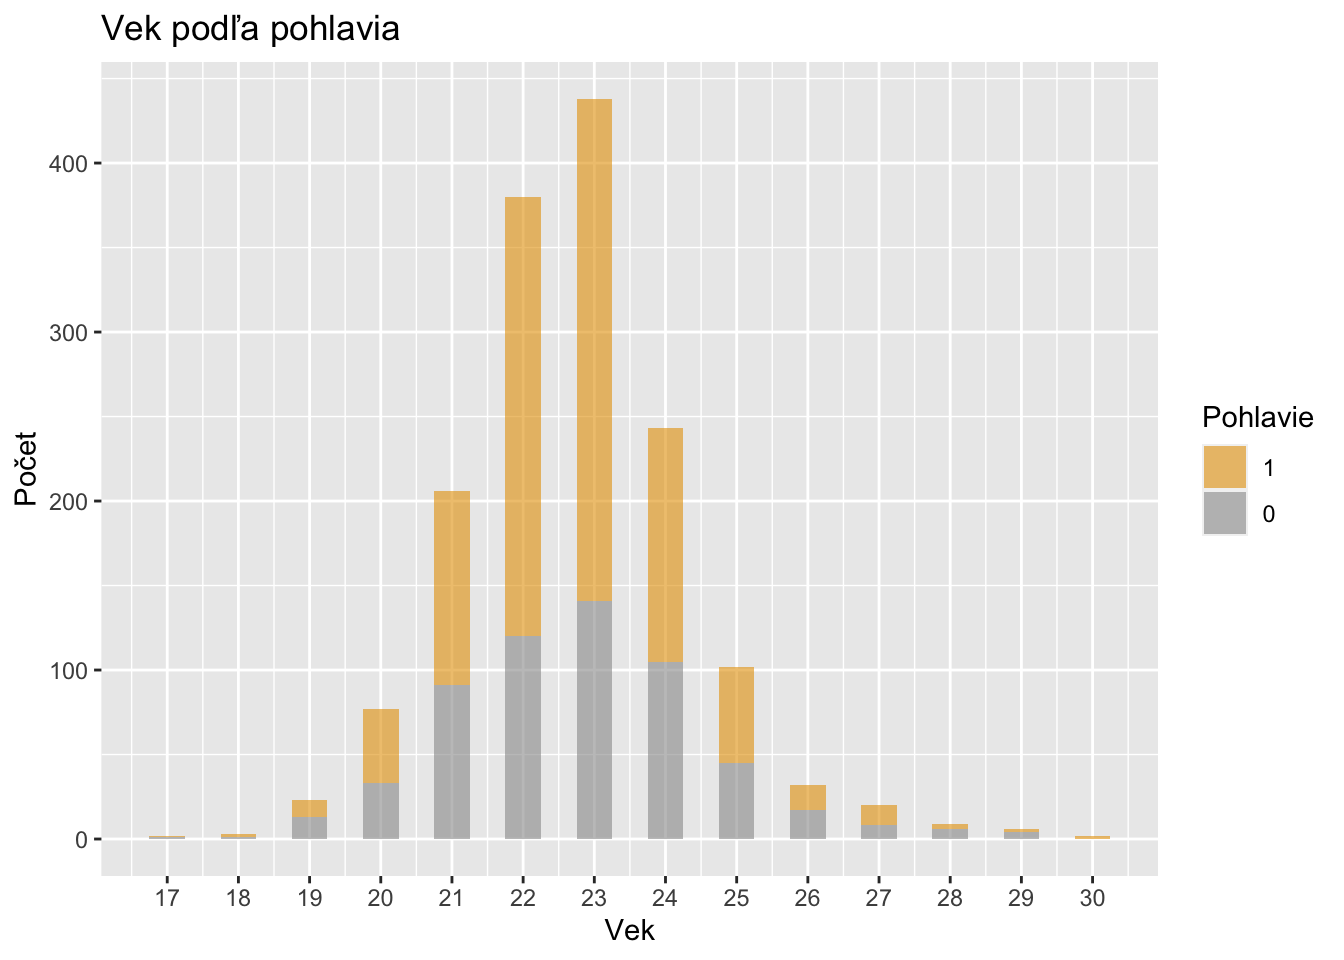
\includegraphics[width=0.8\linewidth,]{_index_files/figure-latex/ageplot-1} 

}

\caption{Distribúcia veku podľa pohlavia}\label{fig:ageplot}
\end{figure}

Z celkovej vzorky, 2,7\% participantov sa hlásilo k etnickej minorite, 3.5\% k sexuálnej menšine (queer), 5,2\% k náboženskej minorite, a po 1,0\% participantov reportovalo postihnutie alebo status imigranta.

Najviac zastúpení vo vzorke boli študenti pochádzajúci z krajov východného Slovenska. V Tabuľke \ref{tab:regionTab} sú zobrazené počty a proporcie participantov podľa kraja, odkiaľ pochádzajú.

\begin{table}[H]

\caption{\label{tab:regionTab}Participanti podľa kraja}
\centering
\fontsize{10}{12}\selectfont
\begin{tabular}[t]{lrr}
\toprule
Región pôvodu participantov & n & percent\\
\midrule
\cellcolor{gray!6}{Prešovský kraj} & \cellcolor{gray!6}{382} & \cellcolor{gray!6}{23.57}\\
Košický kraj & 247 & 15.24\\
\cellcolor{gray!6}{Banskobystrický kraj} & \cellcolor{gray!6}{198} & \cellcolor{gray!6}{12.21}\\
Bratislavský kraj & 189 & 11.66\\
\cellcolor{gray!6}{Žilinský kraj} & \cellcolor{gray!6}{155} & \cellcolor{gray!6}{9.56}\\
\addlinespace
Trnavský kraj & 139 & 8.57\\
\cellcolor{gray!6}{Trenčiansky kraj} & \cellcolor{gray!6}{107} & \cellcolor{gray!6}{6.60}\\
Nitriansky kraj & 75 & 4.63\\
\bottomrule
\end{tabular}
\end{table}

\hypertarget{ux161tudijnuxe9-charakteristiky}{%
\subsection{Študijné charakteristiky}\label{ux161tudijnuxe9-charakteristiky}}

Výskumná vzorka reprezentovala participantov študujúcich všetky skupiny odborov. Tabuľka \ref{tab:regFieldTab} zobrazuje počty participantov vo vzorke podľa lokality fakulty, na ktorej v čase výskumu študovali, zatiaľ čo Tabuľka \ref{tab:fieldStudyTab} zobrazuje počty participantov podľa študijných odborov, ktoré študovali. Najviac zastúpené je západné, najmenej stredné Slovensko. Rozdelenie participantov vo vzorke z hľadiska odborov približne kopíruje populačné proporcie počtu študentov študujúcich dané odbory na Slovensku.

\begin{table}[H]

\caption{\label{tab:regFieldTab}Región fakulty}
\centering
\fontsize{10}{12}\selectfont
\begin{tabular}[t]{lrr}
\toprule
Región fakulty & n & percent\\
\midrule
\cellcolor{gray!6}{Západné Slovensko} & \cellcolor{gray!6}{761} & \cellcolor{gray!6}{46.95}\\
Východné Slovensko & 532 & 32.82\\
\cellcolor{gray!6}{Stredné Slovensko} & \cellcolor{gray!6}{328} & \cellcolor{gray!6}{20.23}\\
\bottomrule
\end{tabular}
\end{table}

\begin{table}[H]

\caption{\label{tab:fieldStudyTab}Skupiny študijných odborov}
\centering
\fontsize{10}{12}\selectfont
\begin{tabular}[t]{lrr}
\toprule
Odbor & n & percent\\
\midrule
\cellcolor{gray!6}{spoločenský, ekonomický, právny} & \cellcolor{gray!6}{505} & \cellcolor{gray!6}{31.15}\\
technický & 412 & 25.42\\
\cellcolor{gray!6}{filozofický, humanitný, pedagogický, teologický} & \cellcolor{gray!6}{351} & \cellcolor{gray!6}{21.65}\\
zdravotnícky & 221 & 13.63\\
\cellcolor{gray!6}{prírodovedecký} & \cellcolor{gray!6}{70} & \cellcolor{gray!6}{4.32}\\
\addlinespace
mediálny, umelecký & 62 & 3.82\\
\bottomrule
\end{tabular}
\end{table}

Nižšie je možné vidieť skupiny odborov rozdelené podľa pohlavia (Graf \ref{fig:fieldPlotMF}) a podľa ročníka (Graf \ref{fig:fieldPlotYear}).

\begin{figure}

{\centering 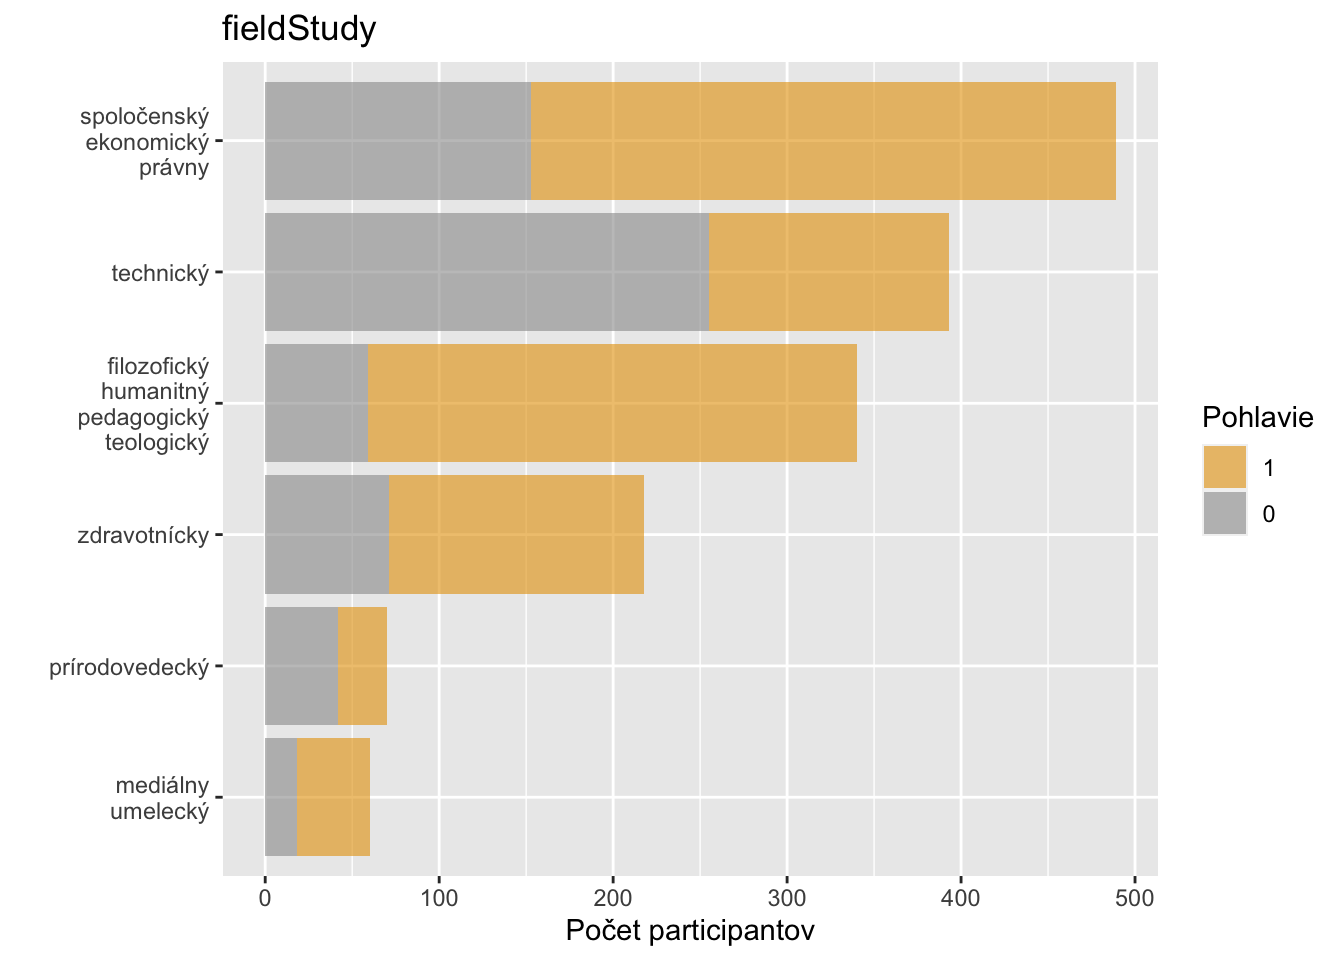
\includegraphics[width=0.8\linewidth,]{_index_files/figure-latex/fieldPlotMF-1} 

}

\caption{Odbor štúdia podľa pohlavia}\label{fig:fieldPlotMF}
\end{figure}

\begin{figure}

{\centering 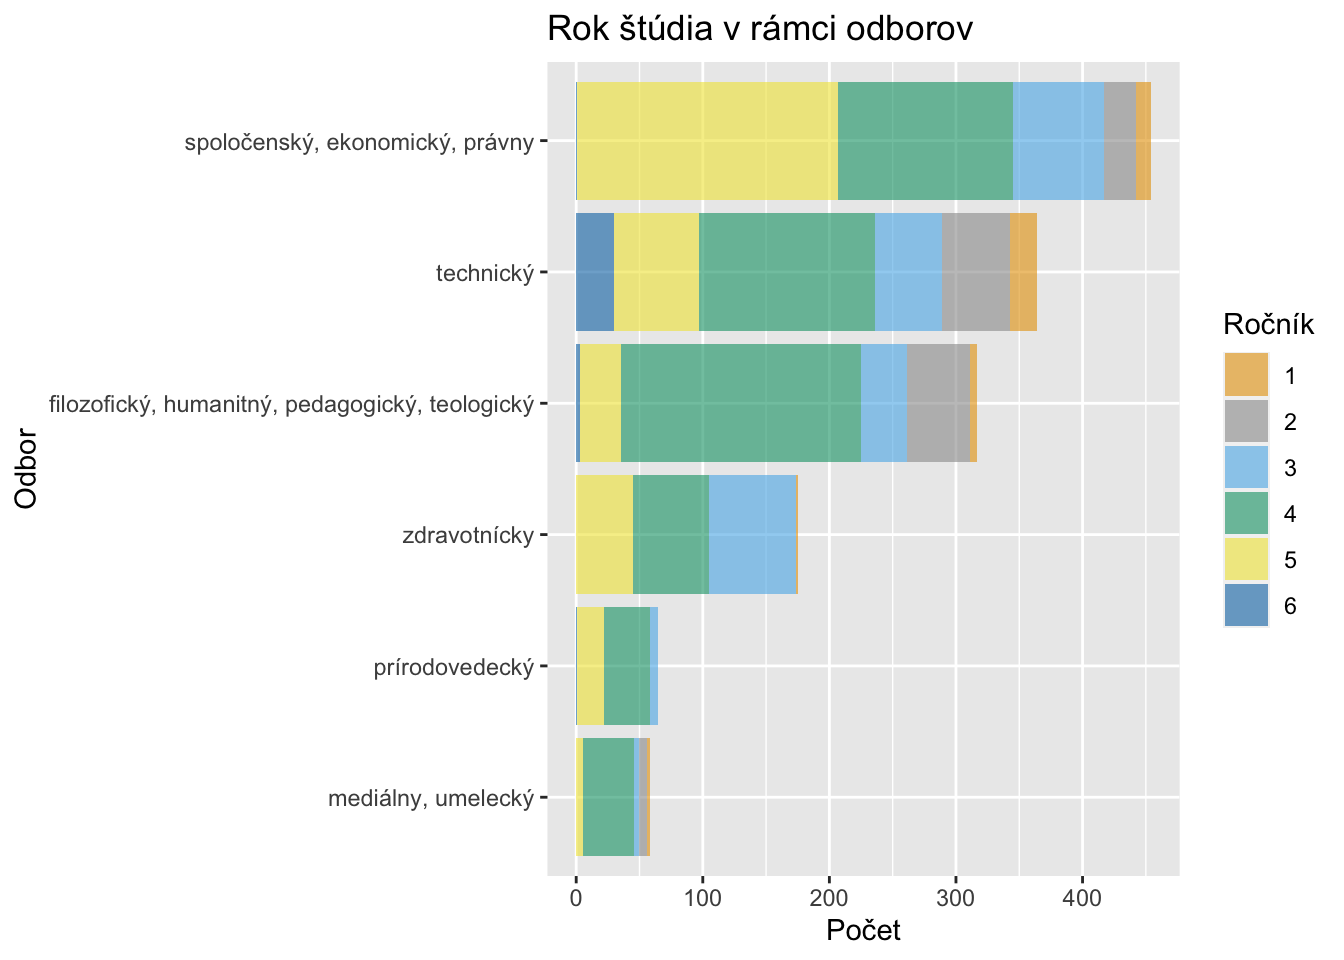
\includegraphics[width=0.8\linewidth,]{_index_files/figure-latex/fieldPlotYear-1} 

}

\caption{Odbor štúdia podľa ročníka}\label{fig:fieldPlotYear}
\end{figure}

\hypertarget{vyluxfaux10denie-nedbanlivuxfdch-participantov}{%
\subsection{Vylúčenie nedbanlivých participantov}\label{vyluxfaux10denie-nedbanlivuxfdch-participantov}}

V následnom kroku boli z celkovej vzorky vylúčení participanti, ktorých štýl odpovedania vykazoval znaky nedbanlivosti. Konkrétne, participant bol z ďalších analýz vylúčený ak sada jeho odpovedí spĺňal aspoň jedno z 5 kritérií uvedenými v sekcii \ref{analyza-dat}. Týmto spôsobo bolo vylúčených \emph{n} = 155, čo predstavuje 10.57\% participantov, redukujúc analytickú vzorku pre nasledujúce analýzy na \emph{n} = 1466. Obdobná miera redukcie vzorky o nedbanlivých participantov býva v podobných výskumných dizajnoch štandardom (Meade \& Craig, 2012).

\newpage

\hypertarget{vysledky}{%
\section{Výsledky výskumu}\label{vysledky}}

\hypertarget{prevalencia-foriem-sexuuxe1lneho-obux165aux17eovania}{%
\subsection{Prevalencia foriem sexuálneho obťažovania}\label{prevalencia-foriem-sexuuxe1lneho-obux165aux17eovania}}

Primárnym výsledkom výskumu sú odhady populačných proporcií jednotlivých foriem sexuálneho obťažovania. Celkovo bolo meraných 20 rôznych foriem sexuálneho obťažovania (ich konkrétna špecifikácia je uvedená v časti ??). Týchto 20 konkrétnych foriem spadá do 3 nadradených klastrov, ktorými sú (1) rodovo motivované obťažovanie (formy 1-8), (2) nechcená sexuálna pozornosť (formy 9-16), a (3) sexuálny nátlak (formy 17-20). Na grafe \ref{fig:prevItems} sú zobrazené vážené percentuálne prevalencie 20 individuálnych foriem, s farebným odlíšením foriem, do ktorých spadajú.

\begin{figure}

{\centering 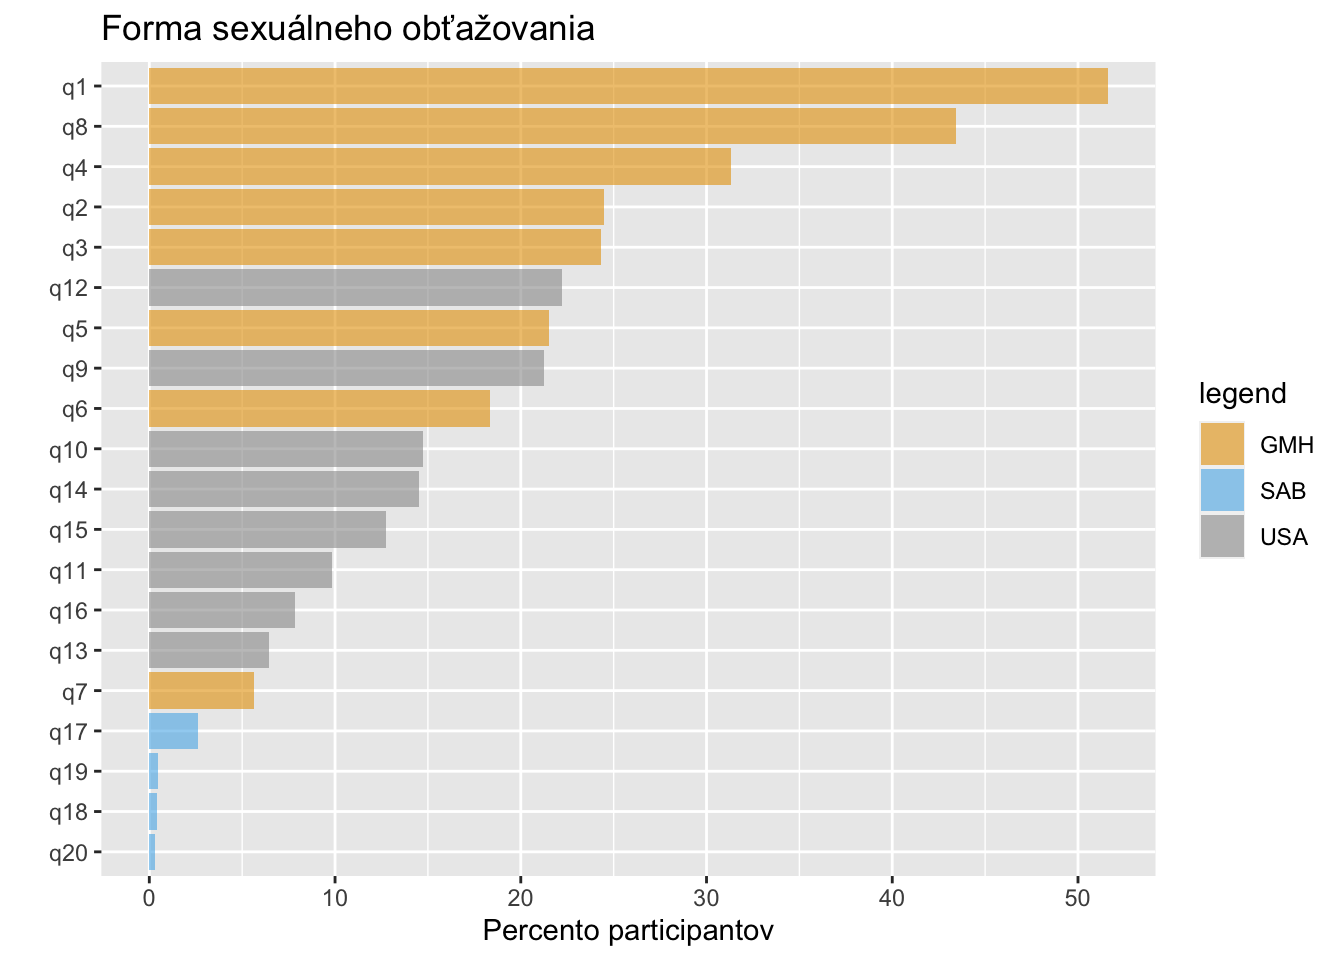
\includegraphics[width=0.8\linewidth,]{_index_files/figure-latex/prevItems-1} 

}

\caption{Prevalencia individuálnych foriem sexuálneho obťažovania}\label{fig:prevItems}
\end{figure}

Prevalencia rodovo motivovaného obťažovania variuje od 5.6\% do 51.6\%, prevalencia foriem nechcenej sexuálnej pozornosti od 6.5\% do 22.2\%, a najmenej frekventovanou formou sexuálneho obťažovania je sexuálne násilie, kde sa prevalencia jednotlivých foriem pohybuje medzi 0.3\% a 2.6\%. Celkovo 76.23\% (\emph{N} = 1134) participantov reportovalo, že zažilo aspoň jednu z foriem rodovo motivovaného obťažovania, 45.98\% (\emph{N} = 666) nechcenú sexuálnu pozornosť a 2.96\% (\emph{N} = 43) sexuálny nátlak.\footnote{Reportované frekvencie reflektujú na rozdiel od percent prirodzené, nie vážené počty participantov-obetí.}

\begin{figure}

{\centering 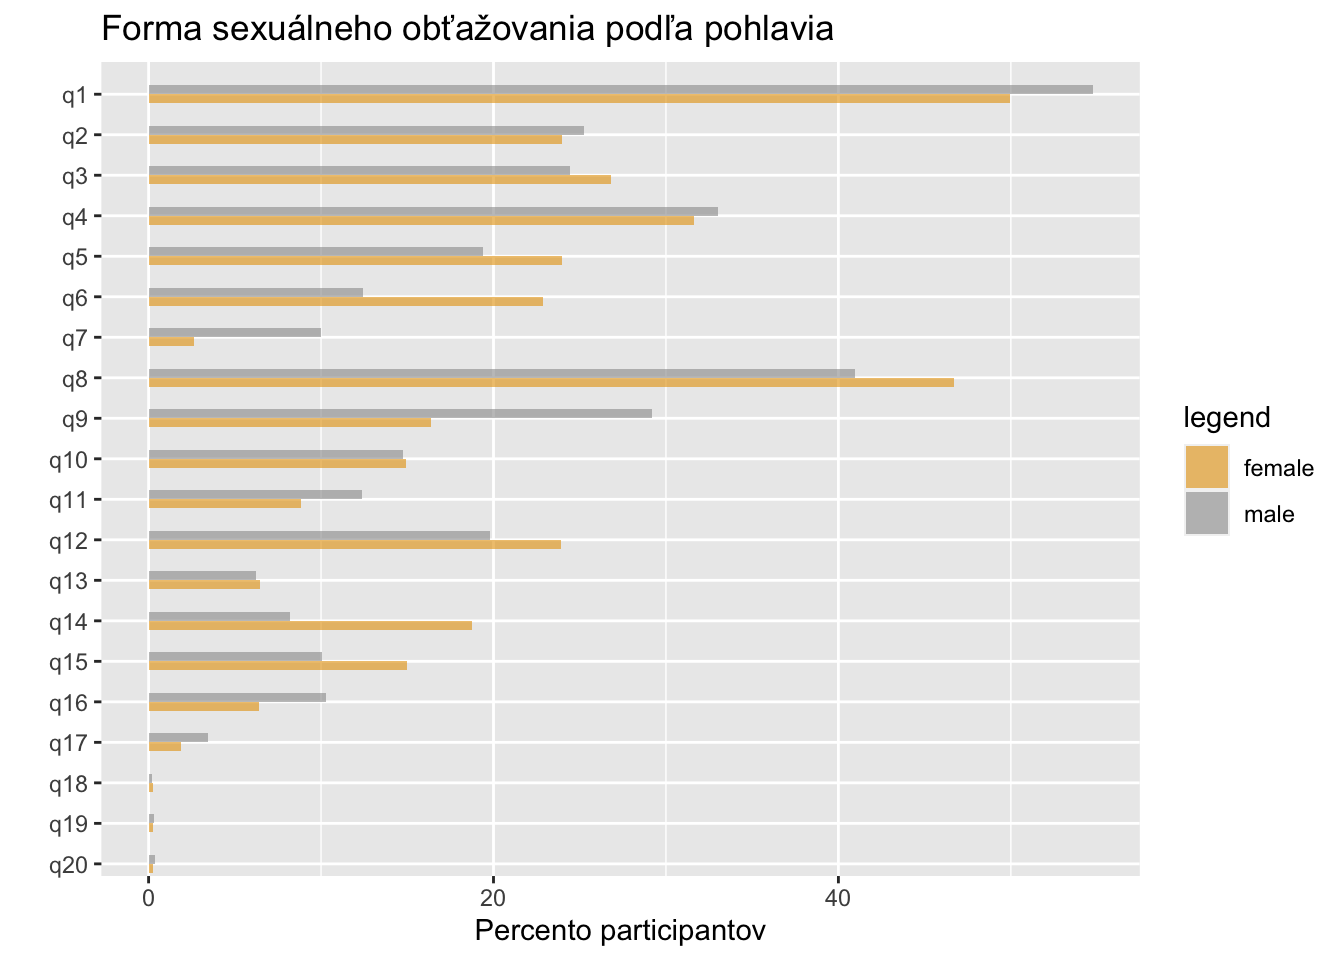
\includegraphics[width=0.8\linewidth,]{_index_files/figure-latex/prevItemsG-1} 

}

\caption{Prevalencia individuálnych foriem sexuálneho obťažovania podľa rodu}\label{fig:prevItemsG}
\end{figure}

Populačné odhady prevalencií pre jednotlivé formy, separátne pre ženy a mužov je možné vidieť na grafe \ref{fig:prevItemsG} a prevalencie sexuálneho obťažovania pre klastre na grafe \ref{fig:prevClust}. Nižšie v tabuľke \ref{tab:prevGenderTab} sú uvedené prevalencie pre ženy a mužov s 95\% intervalmi spoľahlivosti z binomiálneho testu proporcií (založeného na prirodzených výžených počtoch participantov).

\begin{figure}

{\centering 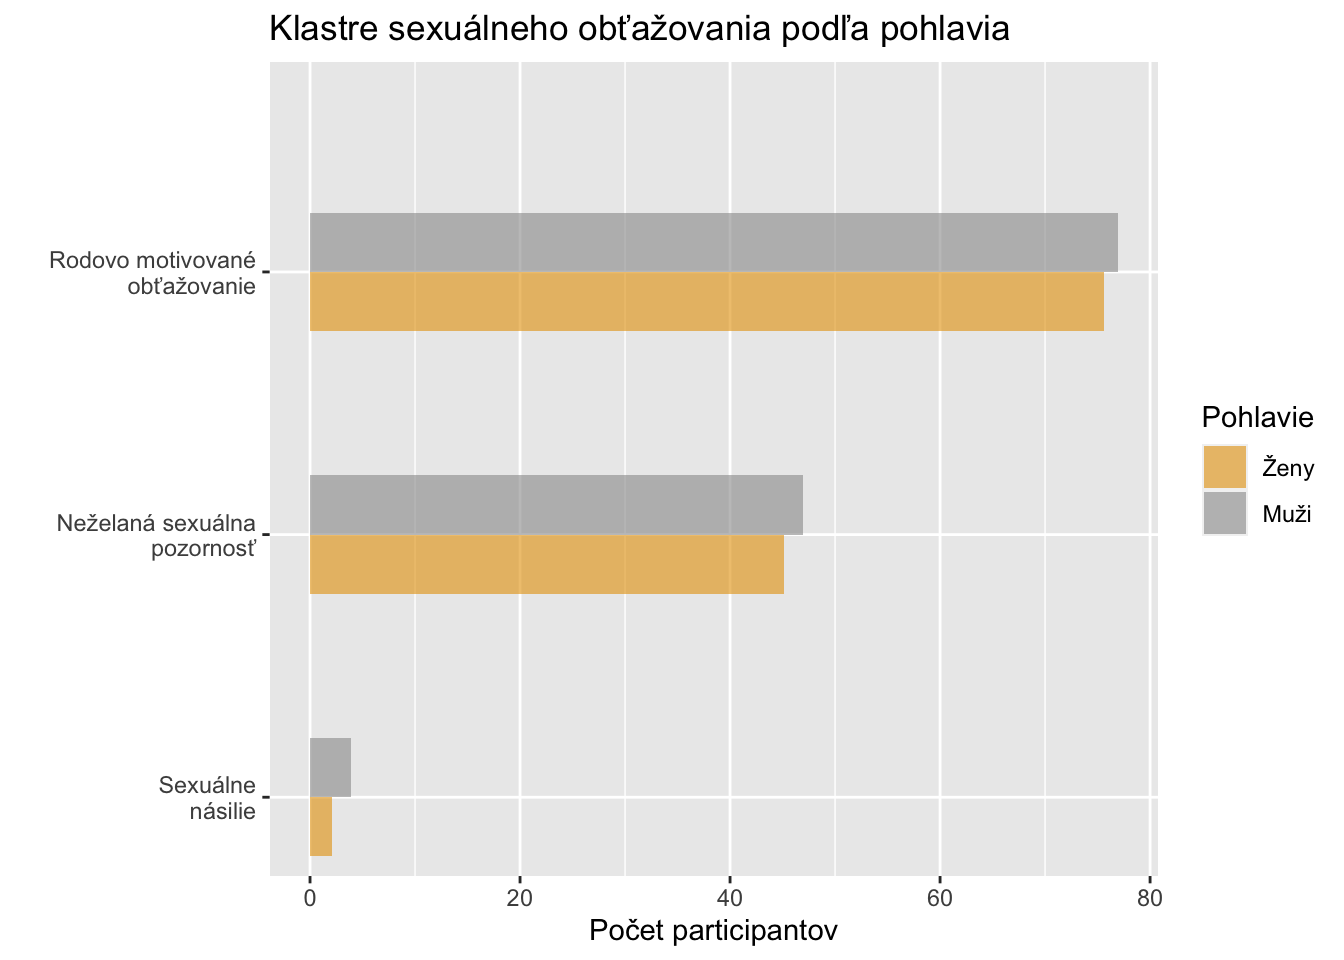
\includegraphics[width=0.8\linewidth,]{_index_files/figure-latex/prevClust-1} 

}

\caption{Prevalencia klastrov sexuálneho obťažovania podľa pohlavia}\label{fig:prevClust}
\end{figure}

\begin{table}[H]

\caption{\label{tab:prevGenderTab}Prevalencie foriem a klastrov sexuálneho obťažovania podľa pohlavia}
\centering
\resizebox{\linewidth}{!}{
\fontsize{10}{12}\selectfont
\begin{tabular}[t]{lrrrlrrr}
\toprule
Forma SO u dievčat & Prevalencia v \% & CI spodný & CI horný & Forma SO u chlapcov & Prevalencia v \% & CI spodný & CI horný\\
\midrule
\cellcolor{gray!6}{q1} & \cellcolor{gray!6}{50.00} & \cellcolor{gray!6}{46.65} & \cellcolor{gray!6}{53.35} & \cellcolor{gray!6}{q1} & \cellcolor{gray!6}{54.79} & \cellcolor{gray!6}{50.54} & \cellcolor{gray!6}{59.00}\\
q2 & 24.00 & 21.20 & 26.97 & q2 & 25.18 & 21.61 & 29.02\\
\cellcolor{gray!6}{q3} & \cellcolor{gray!6}{26.84} & \cellcolor{gray!6}{23.85} & \cellcolor{gray!6}{30.00} & \cellcolor{gray!6}{q3} & \cellcolor{gray!6}{24.34} & \cellcolor{gray!6}{20.74} & \cellcolor{gray!6}{28.22}\\
q4 & 31.60 & 28.48 & 34.85 & q4 & 32.96 & 29.01 & 37.11\\
\cellcolor{gray!6}{q5} & \cellcolor{gray!6}{23.92} & \cellcolor{gray!6}{21.09} & \cellcolor{gray!6}{26.92} & \cellcolor{gray!6}{q5} & \cellcolor{gray!6}{19.36} & \cellcolor{gray!6}{16.09} & \cellcolor{gray!6}{22.98}\\
\addlinespace
q6 & 22.81 & 20.03 & 25.77 & q6 & 12.38 & 9.71 & 15.48\\
\cellcolor{gray!6}{q7} & \cellcolor{gray!6}{2.56} & \cellcolor{gray!6}{1.61} & \cellcolor{gray!6}{3.84} & \cellcolor{gray!6}{q7} & \cellcolor{gray!6}{9.98} & \cellcolor{gray!6}{7.59} & \cellcolor{gray!6}{12.82}\\
q8 & 46.70 & 43.33 & 50.09 & q8 & 40.88 & 36.73 & 45.12\\
\cellcolor{gray!6}{q9} & \cellcolor{gray!6}{16.38} & \cellcolor{gray!6}{13.98} & \cellcolor{gray!6}{19.01} & \cellcolor{gray!6}{q9} & \cellcolor{gray!6}{29.07} & \cellcolor{gray!6}{25.29} & \cellcolor{gray!6}{33.07}\\
q10 & 14.93 & 12.62 & 17.47 & q10 & 14.65 & 11.81 & 17.87\\
\addlinespace
\cellcolor{gray!6}{q11} & \cellcolor{gray!6}{8.82} & \cellcolor{gray!6}{7.01} & \cellcolor{gray!6}{10.91} & \cellcolor{gray!6}{q11} & \cellcolor{gray!6}{12.20} & \cellcolor{gray!6}{9.56} & \cellcolor{gray!6}{15.26}\\
q12 & 23.86 & 21.07 & 26.82 & q12 & 19.82 & 16.55 & 23.41\\
\cellcolor{gray!6}{q13} & \cellcolor{gray!6}{6.47} & \cellcolor{gray!6}{4.92} & \cellcolor{gray!6}{8.32} & \cellcolor{gray!6}{q13} & \cellcolor{gray!6}{6.20} & \cellcolor{gray!6}{4.33} & \cellcolor{gray!6}{8.56}\\
q14 & 18.76 & 16.23 & 21.51 & q14 & 8.06 & 5.92 & 10.67\\
\cellcolor{gray!6}{q15} & \cellcolor{gray!6}{14.93} & \cellcolor{gray!6}{12.62} & \cellcolor{gray!6}{17.47} & \cellcolor{gray!6}{q15} & \cellcolor{gray!6}{10.07} & \cellcolor{gray!6}{7.66} & \cellcolor{gray!6}{12.94}\\
\addlinespace
q16 & 6.29 & 4.78 & 8.11 & q16 & 10.24 & 7.83 & 13.09\\
\cellcolor{gray!6}{q17} & \cellcolor{gray!6}{1.83} & \cellcolor{gray!6}{1.05} & \cellcolor{gray!6}{2.95} & \cellcolor{gray!6}{q17} & \cellcolor{gray!6}{3.46} & \cellcolor{gray!6}{2.10} & \cellcolor{gray!6}{5.35}\\
q18 & 0.23 & 0.03 & 0.82 & q18 & 0.18 & 0.00 & 1.01\\
\cellcolor{gray!6}{q19} & \cellcolor{gray!6}{0.23} & \cellcolor{gray!6}{0.03} & \cellcolor{gray!6}{0.82} & \cellcolor{gray!6}{q19} & \cellcolor{gray!6}{0.18} & \cellcolor{gray!6}{0.00} & \cellcolor{gray!6}{1.02}\\
q20 & 0.23 & 0.03 & 0.82 & q20 & 0.36 & 0.04 & 1.31\\
\addlinespace
\cellcolor{gray!6}{Rodovo motivované obťažovanie} & \cellcolor{gray!6}{75.68} & \cellcolor{gray!6}{72.72} & \cellcolor{gray!6}{78.46} & \cellcolor{gray!6}{Rodovo motivované obťažovanie} & \cellcolor{gray!6}{76.90} & \cellcolor{gray!6}{73.16} & \cellcolor{gray!6}{80.34}\\
Nechcená sexuálna pozornosť & 45.16 & 41.85 & 48.50 & Nechcená sexuálna pozornosť & 46.93 & 42.71 & 51.18\\
\cellcolor{gray!6}{Sexuálny nátlak} & \cellcolor{gray!6}{2.03} & \cellcolor{gray!6}{1.21} & \cellcolor{gray!6}{3.18} & \cellcolor{gray!6}{Sexuálny nátlak} & \cellcolor{gray!6}{3.79} & \cellcolor{gray!6}{2.36} & \cellcolor{gray!6}{5.74}\\
\bottomrule
\end{tabular}}
\end{table}

Z grafu \ref{fig:prevItemsG} je zrejmé, že naprieč formami sexuálneho obťažovania existuje v predmetnej vzorke variabilita v rozdieloch medzi ženami a mužmi. Relevantné však je, či pozorované rozdiely odzrkadľujú reálne existujúce, systematické rozdiely v populácii alebo náhodné fluktuácie. Za účelom odhadu relatívneho rizika a testovania, či je možné zodpovedajúce rozdiely očakávať v celej populácii študentov Slovenských vysokých škôl, bolo pre každú formu sexuálneho obťažovania vypočítané relatívne riziko spolu s 95\% intervalmi spoľahlivosti a Bayesov faktor. Výsledky sú reportované v Tabuľke \ref{tab:rrTable}.

Hodnoty relatívneho rizika väčšie ako 1 vyjadrujú väčšie riziko u žien, hodnoty menšie ako jeden väčšie riziko u mužov. Ak interval spoľahlivosti pretína hodnotu 1, nebol detekovaný štatisticky významný rozdiel v riziku danej formy. Hodnoty Bayesových faktorov na druhej strane predstavujú mieru empirických dôkazov v prospech rozdielu v prevalenciách u žien a mužov. \emph{BF10} vyjadruje mieru dôkazov v prospech alternatívnej hypotézy (existencia rozdielu), \emph{BF01} na druhej strane mieru dôkazov v prospech nulovej hypotézy (absencia rozdielu). Napríklad \emph{BF10} = 2.55 tak znamená, že je 2.55 krát pravdepodobnejšie, že pozorovaný pomer rizík je reálny systematický efekt, zatiaľ čo \emph{BF01} = 7.93 znamená takmer 8x vačšiu pravdepodobnosť, že v populácii neexistuje rozdiel v riziku danej formy sexuálneho obťažovania.

\begin{table}[H]

\caption{\label{tab:rrTable}Relatívne riziko a Bayesove faktory pre rozdiely v prevalencii sexuálneho obťažovania podľa pohlavia}
\centering
\resizebox{\linewidth}{!}{
\fontsize{10}{12}\selectfont
\begin{tabular}[t]{lrrrl}
\toprule
  & Relatívne riziko & CI spodný & CI horný & Bayesov faktor\\
\midrule
\cellcolor{gray!6}{q1} & \cellcolor{gray!6}{0.91} & \cellcolor{gray!6}{0.83} & \cellcolor{gray!6}{1.01} & \cellcolor{gray!6}{BF01 = 1.57}\\
q2 & 0.95 & 0.79 & 1.15 & BF01 = 7.82\\
\cellcolor{gray!6}{q3} & \cellcolor{gray!6}{1.10} & \cellcolor{gray!6}{0.91} & \cellcolor{gray!6}{1.33} & \cellcolor{gray!6}{BF01 = 5.32}\\
q4 & 0.96 & 0.82 & 1.12 & BF01 = 7.09\\
\cellcolor{gray!6}{q5} & \cellcolor{gray!6}{1.24} & \cellcolor{gray!6}{1.01} & \cellcolor{gray!6}{1.54} & \cellcolor{gray!6}{BF01 = 1.18}\\
\addlinespace
q6 & 1.85 & 1.45 & 2.43 & BF10 = 28738.47\\
\cellcolor{gray!6}{q7} & \cellcolor{gray!6}{0.27} & \cellcolor{gray!6}{0.16} & \cellcolor{gray!6}{0.42} & \cellcolor{gray!6}{BF10 = 729539.39}\\
q8 & 1.14 & 1.01 & 1.29 & BF10 = 1.21\\
\cellcolor{gray!6}{q9} & \cellcolor{gray!6}{0.56} & \cellcolor{gray!6}{0.46} & \cellcolor{gray!6}{0.68} & \cellcolor{gray!6}{BF10 = 1143824.32}\\
q10 & 1.01 & 0.78 & 1.31 & BF01 = 10.83\\
\addlinespace
\cellcolor{gray!6}{q11} & \cellcolor{gray!6}{0.72} & \cellcolor{gray!6}{0.52} & \cellcolor{gray!6}{0.98} & \cellcolor{gray!6}{BF01 = 1.4}\\
q12 & 1.21 & 0.99 & 1.50 & BF01 = 1.72\\
\cellcolor{gray!6}{q13} & \cellcolor{gray!6}{1.03} & \cellcolor{gray!6}{0.69} & \cellcolor{gray!6}{1.59} & \cellcolor{gray!6}{BF01 = 15.62}\\
q14 & 2.29 & 1.71 & 3.19 & BF10 = 861678.27\\
\cellcolor{gray!6}{q15} & \cellcolor{gray!6}{1.50} & \cellcolor{gray!6}{1.12} & \cellcolor{gray!6}{2.05} & \cellcolor{gray!6}{BF10 = 3.61}\\
\addlinespace
q16 & 0.62 & 0.43 & 0.88 & BF10 = 2.62\\
\cellcolor{gray!6}{q17} & \cellcolor{gray!6}{0.52} & \cellcolor{gray!6}{0.26} & \cellcolor{gray!6}{1.01} & \cellcolor{gray!6}{BF01 = 3.5}\\
q18 & 1.29 & 0.00 & Inf & BF01 = 78.01\\
\cellcolor{gray!6}{q19} & \cellcolor{gray!6}{0.64} & \cellcolor{gray!6}{0.00} & \cellcolor{gray!6}{Inf} & \cellcolor{gray!6}{BF01 = 60.89}\\
q20 & 0.65 & 0.00 & Inf & BF01 = 61.53\\
\addlinespace
\cellcolor{gray!6}{Rodovo motivované obťažovanie} & \cellcolor{gray!6}{0.98} & \cellcolor{gray!6}{0.93} & \cellcolor{gray!6}{1.04} & \cellcolor{gray!6}{BF01 = 7.73}\\
Nechcená sexuálna pozornosť & 0.96 & 0.86 & 1.08 & BF01 = 6.15\\
\cellcolor{gray!6}{Sexuálny nátlak} & \cellcolor{gray!6}{0.56} & \cellcolor{gray!6}{0.29} & \cellcolor{gray!6}{1.04} & \cellcolor{gray!6}{BF01 = 3.84}\\
\bottomrule
\end{tabular}}
\end{table}

Štatisticky signifikantný rozdiel medzi pohlaviami v riziku výskytu danej formy sexuálneho obťažovania bol zaznamenaný v nasledujúcich formách (prezentované z pohľadu žien): forma q5 o 24\% väčšie riziko no miera dôkazov v prospech existencie rozdielu je veľmi slabá (\emph{BF01} = 1.17); q6 1.85x vačšie riziko a q7 o \textasciitilde73\% menšie riziko, pričom oba efekty sú veľmi robustné; q8 o 14\% väčšie riziko no miera dôkazov v prospech rozdielu je mimoriadne slabá; q9 o 44\% menšie riziko - veľmi silný efekt; q11 o 28\% mensie riziko no miera dôkazov v prospech tvrdenia je mimoriadne slabá; v prípade formy q14 bolo zistené 2.29x vačšie riziko, pričom sa jedná o veľmi robustný efekt; q15 o 50\% vačšie riziko no miera dôkazov je slabá (hypotéza existencie rozdielu je iba 3.73x pravdepodobnejšia ako nulová hypotéza), q16 o 38\% menšie riziko no miera dôkazov je podobne slabá (\emph{BF10} = 2.55). Pri ostatných individuálnych formách nebol štatisticky signifikantný rozdiel. Najmä pri formách sexuálneho nátlaku (q17 - q20) boli frekvencie reportovaných prípadov tak nízke, že pomer rizík nebol interpretovateľný a nebolo ani možné odhadnúť informatívny interval spoľahlivosti.

Z hľadiska klastrov sexuálneho obťažovania nebol ani v jednom pozorovaný signifikantný rozdiel medzi pohlaviami. Hodnoty Bayesovho faktora v prospech nulovej hypotézy (\emph{BF01}) pre dané tri klastre boli na úrovni 7.73, 6.42 a 3.89, čiže skôr bola detekovaná absencia rozdielov v riziku daného klastra u participantov.

\hypertarget{rizikovuxe9-faktory-sexuuxe1lneho-obux165aux17eovania}{%
\subsection{Rizikové faktory sexuálneho obťažovania}\label{rizikovuxe9-faktory-sexuuxe1lneho-obux165aux17eovania}}

Keďže v mnohých formách sexuálneho obťažovania boli zaznamenané výraznejšie prevalencie, v ďalšom kroku sme sa zamerali na skúmanie rizikových faktorov agregátnych foriem (klastrov) sexuálneho obťažovania. V Tabuľkách \ref{tab:rfGMH}, \ref{tab:rfUSA}, resp. \ref{tab:rfSAB} sú reportované hodnoty relatívneho rizika a Bayesove faktory pre dichotomické rizikové faktory troch klastrov sexuálneho obťažovania. Ako je možné vidieť, hodnoty relatívneho rizika pre jednotlivé faktory pri veľkej väčšine faktorov blízke 1, resp. interval spoľahlivosti zahŕňa 1 (rovnaké riziko pre obe úrovne rizikového faktora). Signifikantné hodnoty relatívneho rizika boli zaznamenané iba v nasledujúcich prípadoch: vek vyšší ako 23 rokov bol asociovaný s mierne nižším rizikom rodovo motivovaného obťažovania (o 9\%, \emph{BF10} = 10.9), neheterosexuálna orientácia bola asociovaná s 35\% vyšším rizikom nechcenej sexuálnej pozornosti (no \emph{BF10} = 1.01, takže miera empirických dôkazov v prospech alternatívnej hypotézy prakticky absentuje). Po zohľadnení inflácie miery chyby I. typu v dôsledku viacnásobného testovania (korigovaním hladiny \(\alpha\) Bonferroniho korekciou), ostal signifikantným iba efekt veku pri rodovo motivovanom obťažovaní.

\begin{table}[H]

\caption{\label{tab:rfGMH}Rodovo motivované obťažovanie - rizikové faktory}
\centering
\resizebox{\linewidth}{!}{
\fontsize{10}{12}\selectfont
\begin{tabular}[t]{lrrrl}
\toprule
  & Relatívne riziko & CI spodný & CI horný & Bayesov faktor\\
\midrule
\cellcolor{gray!6}{Rod} & \cellcolor{gray!6}{0.98} & \cellcolor{gray!6}{0.93} & \cellcolor{gray!6}{1.04} & \cellcolor{gray!6}{BF01 = 7.73}\\
Neheterosexuál & 1.00 & 0.86 & 1.14 & BF01 = 22.21\\
\cellcolor{gray!6}{Minorita} & \cellcolor{gray!6}{1.01} & \cellcolor{gray!6}{0.92} & \cellcolor{gray!6}{1.10} & \cellcolor{gray!6}{BF01 = 14.32}\\
Vek viac ako 23 & 0.92 & 0.86 & 0.97 & BF10 = 10.37\\
\cellcolor{gray!6}{Veriaci} & \cellcolor{gray!6}{1.00} & \cellcolor{gray!6}{0.94} & \cellcolor{gray!6}{1.07} & \cellcolor{gray!6}{BF01 = 10.38}\\
\addlinespace
Iný materinský jazyk & 0.96 & 0.87 & 1.06 & BF01 = 10.54\\
\bottomrule
\end{tabular}}
\end{table}
\begin{table}[H]

\caption{\label{tab:rfUSA}Nechcená sexuálna pozornosť - rizikové faktory}
\centering
\resizebox{\linewidth}{!}{
\fontsize{10}{12}\selectfont
\begin{tabular}[t]{lrrrl}
\toprule
  & Relatívne riziko & CI spodný & CI horný & Bayesov faktor\\
\midrule
\cellcolor{gray!6}{Rod} & \cellcolor{gray!6}{0.96} & \cellcolor{gray!6}{0.86} & \cellcolor{gray!6}{1.08} & \cellcolor{gray!6}{BF01 = 6.15}\\
Neheterosexuál & 1.35 & 1.07 & 1.63 & BF01 = 1.01\\
\cellcolor{gray!6}{Minorita} & \cellcolor{gray!6}{0.96} & \cellcolor{gray!6}{0.78} & \cellcolor{gray!6}{1.14} & \cellcolor{gray!6}{BF01 = 11.22}\\
Vek viac ako 23 & 0.90 & 0.81 & 1.01 & BF01 = 1.46\\
\cellcolor{gray!6}{Veriaci} & \cellcolor{gray!6}{0.91} & \cellcolor{gray!6}{0.81} & \cellcolor{gray!6}{1.03} & \cellcolor{gray!6}{BF01 = 2.95}\\
\addlinespace
Iný materinský jazyk & 0.88 & 0.70 & 1.05 & BF01 = 5.06\\
\bottomrule
\end{tabular}}
\end{table}
\begin{table}[H]

\caption{\label{tab:rfSAB}Sexuálny nátlak - rizikové faktory}
\centering
\resizebox{\linewidth}{!}{
\fontsize{10}{12}\selectfont
\begin{tabular}[t]{lrrrl}
\toprule
  & Relatívne riziko & CI spodný & CI horný & Bayesov faktor\\
\midrule
\cellcolor{gray!6}{Rod} & \cellcolor{gray!6}{0.56} & \cellcolor{gray!6}{0.29} & \cellcolor{gray!6}{1.04} & \cellcolor{gray!6}{BF01 = 3.84}\\
Neheterosexuál & 1.81 & 0.00 & 4.41 & BF01 = 27.96\\
\cellcolor{gray!6}{Minorita} & \cellcolor{gray!6}{1.33} & \cellcolor{gray!6}{0.39} & \cellcolor{gray!6}{2.72} & \cellcolor{gray!6}{BF01 = 26.54}\\
Vek viac ako 23 & 0.90 & 0.49 & 1.70 & BF01 = 21\\
\cellcolor{gray!6}{Veriaci} & \cellcolor{gray!6}{1.71} & \cellcolor{gray!6}{0.85} & \cellcolor{gray!6}{5.21} & \cellcolor{gray!6}{BF01 = 11.4}\\
\addlinespace
Iný materinský jazyk & 1.14 & 0.23 & 2.43 & BF01 = 33.63\\
\bottomrule
\end{tabular}}
\end{table}

Zároveň boli analyzované ďalšie 3 multinominálne rizikové faktory: rok štúdia, odbor štúdia a lokalita fakulty, separátne pre všetky tri klastre sexuálneho obťažovania. Bayesiánska analýza ukázala, že jediným robustným efektom je rozdielne riziko rodovo motivovaného obťažovania v závislosti od odboru štúdia (BF10 = 530.67). V porovnaní s referenčnou skupinou študentov filozofických, humanitných, pedagogických, alebo teologických odborov bolo zistené vyššie riziko u študentov zdravotníckych odborov (o 32\%), technických odborov (o 21\%), prírodovedeckých odborov (o 18\%), skupiny spoločenských, ekonomických alebo právnych odborov (o 13\%) a skupiny mediálnych a umeleckých odborov (o 13\%).
Pri ostatných kombináciách formiem sexuálneho obťažovania a rizikových faktorov sme nedetekovali efekt v prospech ktorého by existovalo dostatočné množstvo dôkazov a hodnoty Bayesových faktorov svedčili skôr o absencii efektov (\emph{BF01} v rozmedzí od 2 do 20432).

Ako súhrnnejšiu alternatívu sme analyzovali, či rizikové faktory dokážu predikovať závažnosť sexuálneho obťažovania. Táto premenná reflektuje na jednej strane najzávažnejšiu formu sexuálneho obťažovania, ktorú respondent zažil a na druhej strane jeho frekvenciu.\footnote{Premenná bola kódovaná ako 0 pre participantov, ktorí nereportovali žiadnu formu sexuálneho obťažovania, 1 v prípade jednorázového rodovo motivovaného obťažovania, 2 v prípade opakovaného rodovo motivovaného obťažovania, 3 v prípade jednorázovej nechcenej sexuálnej pozornosti \ldots, a 6 v prípade opakovaného sexuálneho nátlaku.} Ako mierne významný rizikový faktor závažnosti sexuálneho obťažovania sa ukázala sexuálna orientácia, F(1, 1434) = 8.01, p = 0, BF10 = 5.06. Vyšší ročník štúdia bol pozitívne asociovaný so závažnosťou sexuálneho obťažovania, no veľkoť efektu bola malá, \emph{r} = 0.09, podobne ako miera dôkazov v prospech tohto efektu F(1, 1331) = 5.38, p = 0.02, BF10 = 1.36. Celkovo nebol detekovaný efekt regiónu na závažnosť sexuálneho obťažovania, F(2, 1463) = 0.15, p = 0.86, BF01 = 56.54. Podobne nulový populačný efekt mal status príslušníka menšiny, F(1, 1464) = 0, p = 0.95, BF01 = 10.28; viera v Boha, F(1, 1464) = 1.88, p = 0.17, BF01 = 5.5; či používanie iného materinského jazyka ako slovenčiny, F(1, 1464) = 2.31, p = 0.13, BF01 = 2.13.

\hypertarget{puxe1chatelia-sexuuxe1lneho-obux165aux17eovania}{%
\subsection{Páchatelia sexuálneho obťažovania}\label{puxe1chatelia-sexuuxe1lneho-obux165aux17eovania}}

V prípade, že participant sa identifikoval ako obeť konkrétnej formy sexuálneho obťažovania, mal možnosť označiť páchateľa (prípadne páchateľov) danej formy obťažovania. Celkovo, najčastejším páchateľom sexuálneho obťažovania sú študent-muž (37.48\%), učiteľ-muž (24.45\%) a študent-žena (23.17\%). V porovnaní so ženami, u mužov je riziko páchania sexuálneho obťažovania takmer 2x vyššie, RR = 1.88, 95\%CI (1.79, 1.97), p \textless{} .001, BF10 = 1.25e+156. Ide o veľmi robustný efekt. Z hľadiska jednotlivých klastrov sexuálneho obťažovania, muži sú približne dva krát náchylnejší páchať formy rodovo motivovaného obťažovania, RR = 2.03, 95\%CI (1.92, 2.14), p \textless{} .001, BF10 = 2.19e+154 a zároveň aj nechcenej sexuálnej pozornosti RR = 1.61, 95\%CI (1.47, 1.76), p \textless{} .001, BF10 = 6.1e+20. V oblasti sexuálneho násilia nebol z hľadiska pohlavia páchateľa detekovaný signifikantný rozdiel, RR = 0.77, 95\%CI (0.47, 1.24), p = 0.282, BF01 = 392.72.

\begin{table}[H]

\caption{\label{tab:perpClust}Najčastejší páchatelia celkovo - klastre}
\centering
\resizebox{\linewidth}{!}{
\fontsize{10}{12}\selectfont
\begin{tabular}[t]{lrrrrrr}
\toprule
  & Učiteľ Muž & Učiteľ Žena & Študent Muž & Študent Žena & Zamestnanec Muž & Zamestnanec Žena\\
\midrule
\cellcolor{gray!6}{Rodovo motivované obťažovanie} & \cellcolor{gray!6}{30.49} & \cellcolor{gray!6}{11.40} & \cellcolor{gray!6}{32.75} & \cellcolor{gray!6}{19.56} & \cellcolor{gray!6}{3.72} & \cellcolor{gray!6}{2.08}\\
Nechcená sexuálna pozornosť & 9.16 & 3.75 & 50.24 & 32.24 & 2.25 & 2.36\\
\cellcolor{gray!6}{Sexuálny nátlak} & \cellcolor{gray!6}{11.59} & \cellcolor{gray!6}{10.14} & \cellcolor{gray!6}{26.09} & \cellcolor{gray!6}{31.88} & \cellcolor{gray!6}{5.80} & \cellcolor{gray!6}{14.49}\\
\bottomrule
\end{tabular}}
\end{table}

V tabuľke \ref{tab:perpClust} sú pre každý klaster sexuálneho obťažovania uvedené vážené proporcie reportovaných páchateľov. V rámci jednotlivých klastrov sexuálneho obťažovania, rodovo motivovaného obťažovania sa najčastejšie dopúšťajú študenti a učitelia\footnote{Frekvencia kontaktov študentov s učiteľmi a inými študentmi nie je ale rovnomerná. Celkovo, učitelia predstavujú páchateľa sexuálneho obťažovania až v 34\% prípadov. Daný údaj je tak potrebné vnímať v kontexte nízkeho relatívneho zastúpenia učiteľov v štruktúre kontaktov študentov.} mužského pohlavia (33\%, resp. 30\%), na nechcenej sexuálnej pozornosti sa najviac podieľajú študenti a študentky (50\%, resp. 32\%), a najčastejšími páchateľmi sexuálneho donútenia sú v prakticky rovnakej miere študenti a študentky (26\%, resp. 32\%). Nižšie v tabuľkách \ref{tab:perpClustF} a \ref{tab:perpClustM} sú uvedení najčastejší páchatelia pre obete ženského, resp. mužského pohlavia.

\begin{table}[H]

\caption{\label{tab:perpClustF}Najčastejší páchatelia u žien - klastre}
\centering
\resizebox{\linewidth}{!}{
\fontsize{10}{12}\selectfont
\begin{tabular}[t]{lrrrrrr}
\toprule
  & Učiteľ Muž & Učiteľ Žena & Študent Muž & Študent Žena & Zamestnanec Muž & Zamestnanec Žena\\
\midrule
\cellcolor{gray!6}{Rodovo motivované obťažovanie} & \cellcolor{gray!6}{35.99} & \cellcolor{gray!6}{10.27} & \cellcolor{gray!6}{32.15} & \cellcolor{gray!6}{17.42} & \cellcolor{gray!6}{3.23} & \cellcolor{gray!6}{0.94}\\
Nechcená sexuálna pozornosť & 14.05 & 0.49 & 68.29 & 13.66 & 3.41 & 0.10\\
\cellcolor{gray!6}{Sexuálny nátlak} & \cellcolor{gray!6}{32.14} & \cellcolor{gray!6}{0.00} & \cellcolor{gray!6}{53.57} & \cellcolor{gray!6}{0.00} & \cellcolor{gray!6}{14.29} & \cellcolor{gray!6}{0.00}\\
\bottomrule
\end{tabular}}
\end{table}

\begin{table}[H]

\caption{\label{tab:perpClustM}Najčastejší páchatelia u mužov - klastre}
\centering
\resizebox{\linewidth}{!}{
\fontsize{10}{12}\selectfont
\begin{tabular}[t]{lrrrrrr}
\toprule
  & Učiteľ Muž & Učiteľ Žena & Študent Muž & Študent Žena & Zamestnanec Muž & Zamestnanec Žena\\
\midrule
\cellcolor{gray!6}{Rodovo motivované obťažovanie} & \cellcolor{gray!6}{23.87} & \cellcolor{gray!6}{12.90} & \cellcolor{gray!6}{33.66} & \cellcolor{gray!6}{22.23} & \cellcolor{gray!6}{3.98} & \cellcolor{gray!6}{3.37}\\
Nechcená sexuálna pozornosť & 2.32 & 6.56 & 28.96 & 56.76 & 1.16 & 4.25\\
\cellcolor{gray!6}{Sexuálny nátlak} & \cellcolor{gray!6}{0.00} & \cellcolor{gray!6}{3.70} & \cellcolor{gray!6}{7.41} & \cellcolor{gray!6}{70.37} & \cellcolor{gray!6}{0.00} & \cellcolor{gray!6}{18.52}\\
\bottomrule
\end{tabular}}
\end{table}

\hypertarget{miesto-sexuuxe1lneho-obux165aux17eovania}{%
\subsection{Miesto sexuálneho obťažovania}\label{miesto-sexuuxe1lneho-obux165aux17eovania}}

Popri páchateľoch sexuálneho obťažovania, participanti mali pri každej individuálnej forme možnosť uviesť miesto, kde sa daná forma sexuálneho obťažovania udiala. Vo všeobecnosti, sexuálne obťažovanie sa najčastejšie deje počas na škole počas vyučovania a v rámci prestávok (28\%, resp. 28\%), ako aj na internátoch (19\%\%). Dáta separátne pre ženy a mužov je možné vidieť v tabuľke \ref{tab:whereOverall}.

Nižšie taktiež uvádzame dáta podľa jednotlivých klastrov sexuálneho obťažovania (Tabuľka \ref{tab:whereTable}). Z hľadiska klastrov sexuálneho obťažovania, rodovo motivované obťažovanie sa najčastejšie vyskytuje počas edukačného procesu a v rámci prestávok. Nechcená sexuálna pozornosť sa najčastejšie deje v prostredí prestávok a internátov. Sexuálne donútenie sa taktiež najčastejšie odohráva na internáte a počas prestávok.

\begin{table}[H]

\caption{\label{tab:whereOverall}Miesto sexuálneho obťažovania}
\centering
\resizebox{\linewidth}{!}{
\fontsize{10}{12}\selectfont
\begin{tabular}[t]{lrrrrrrr}
\toprule
  & Výučba & Prestávka & Internát & Laboratórium & Prax & Online & Neviem\\
\midrule
\cellcolor{gray!6}{Celkovo} & \cellcolor{gray!6}{28.29} & \cellcolor{gray!6}{27.89} & \cellcolor{gray!6}{19.37} & \cellcolor{gray!6}{2.31} & \cellcolor{gray!6}{3.78} & \cellcolor{gray!6}{12.18} & \cellcolor{gray!6}{6.18}\\
Ženy & 31.18 & 29.25 & 17.74 & 0.78 & 2.51 & 11.81 & 6.73\\
\cellcolor{gray!6}{Muži} & \cellcolor{gray!6}{25.35} & \cellcolor{gray!6}{26.78} & \cellcolor{gray!6}{21.71} & \cellcolor{gray!6}{3.43} & \cellcolor{gray!6}{4.66} & \cellcolor{gray!6}{12.30} & \cellcolor{gray!6}{5.76}\\
\bottomrule
\end{tabular}}
\end{table}

\begin{table}[H]

\caption{\label{tab:whereTable}Miesto sexuálneho obťažovania}
\centering
\resizebox{\linewidth}{!}{
\fontsize{10}{12}\selectfont
\begin{tabular}[t]{lrrrrrrr}
\toprule
  & Výučba & Prestávka & Internát & Laboratórium & Prax & Online & Neviem\\
\midrule
\cellcolor{gray!6}{Rodovo motivované obťažovanie} & \cellcolor{gray!6}{34.54} & \cellcolor{gray!6}{26.70} & \cellcolor{gray!6}{15.45} & \cellcolor{gray!6}{2.20} & \cellcolor{gray!6}{3.49} & \cellcolor{gray!6}{10.22} & \cellcolor{gray!6}{7.41}\\
Nechcená sexuálna pozornosť & 15.57 & 30.68 & 27.51 & 2.40 & 4.16 & 16.18 & 3.51\\
\cellcolor{gray!6}{Sexuálny nátlak} & \cellcolor{gray!6}{18.10} & \cellcolor{gray!6}{20.95} & \cellcolor{gray!6}{21.90} & \cellcolor{gray!6}{5.71} & \cellcolor{gray!6}{9.52} & \cellcolor{gray!6}{15.24} & \cellcolor{gray!6}{8.57}\\
\bottomrule
\end{tabular}}
\end{table}

\hypertarget{subjektuxedvne-duxf4sledky-sexuuxe1lneho-obux165aux17eovania}{%
\subsection{Subjektívne dôsledky sexuálneho obťažovania}\label{subjektuxedvne-duxf4sledky-sexuuxe1lneho-obux165aux17eovania}}

V dôsledku sexuálneho obťažovania, obete reportovali nasledujúce, subjektívne vnímané psychické alebo psychosomatické problémy. Spomedzi skupiny obetí sexuálneho obťažovania, najvačšie percento študentov zažívalo pocity zraniteľnosti, stratu sebaistoty, alebo sa u nich vyvinula subjektívna úzkosť. Niektorí študenti taktiež reportovali problémy s koncentráciou alebo pocity bezmocnosti, depresívne stavy, vzťahové problémy, ťažkosti s učením alebo spánkom, a poruchy príjmu potravy. Detailnejšie dáta rozdelené podľa rodu sú uvedené v Tabuľke \ref{tab:suffer}. Celkovo sa však študenti z hľadiska pohlavia nelíšili v závažnosti (a zároveň rozsahu) uvádzaných dôsledkov, F(1, 1157) = 2.55, p = 0.11, BF01 = 5.42.

Dáta ale indikujú, že rozsah uvádzaných dôsledkov je asociovaný so závažnosťou zažitého sexuálneho obťažovania. Napriek tomu, že veľkosť daného efektu je skôr striedma \emph{r} = 0.13, \emph{p} \textless{} .001, efekt je empiricky značne robustný, BF10 = 24384. Dá sa teda predpokladať, že obete sexuálneho obťažovania majú častejšie následky na mentálnom zdraví. Na druhej strane však rozsah uvádzaných dôsledkov nebol podmienený tým, kto bol u daného participanta najčastejším páchateľom najzávažnejšej formy sexuálneho obťažovania, F(2, 1175) = 0.27, p = 0.76, BF01 = 9.37. Zároveň, nebol zistený vzťah medzi závažnosťou uvádzaných dôsledkov a (1) príslušnosťou k niektorej menšine, F(1, 1176) = 0, p = 0.99, BF01 = 9.55, alebo (2), vierovyznaním F(1, 1176) = 1.87, p = 0.17, BF01 = 12.12.

\begin{table}[H]

\caption{\label{tab:suffer}Subjektívne dôsledky sexuálneho obťažovania}
\centering
\resizebox{\linewidth}{!}{
\fontsize{10}{12}\selectfont
\begin{tabular}[t]{lrrlrrlrr}
\toprule
Celkovo & N & \% & Ženy & N & \% & Muži & N & \%\\
\midrule
\cellcolor{gray!6}{Pocity zraniteľnosti} & \cellcolor{gray!6}{87} & \cellcolor{gray!6}{7} & \cellcolor{gray!6}{Pocity zraniteľnosti} & \cellcolor{gray!6}{71} & \cellcolor{gray!6}{10} & \cellcolor{gray!6}{Strata sebaistoty} & \cellcolor{gray!6}{24} & \cellcolor{gray!6}{5}\\
Strata sebaistoty & 66 & 6 & Strata sebaistoty & 42 & 6 & Ťažkosti s učením & 22 & 5\\
\cellcolor{gray!6}{Úzkosť} & \cellcolor{gray!6}{59} & \cellcolor{gray!6}{5} & \cellcolor{gray!6}{Úzkosť} & \cellcolor{gray!6}{39} & \cellcolor{gray!6}{6} & \cellcolor{gray!6}{Problémy s koncentráciou} & \cellcolor{gray!6}{18} & \cellcolor{gray!6}{4}\\
Problémy s koncentráciou & 47 & 4 & Pocity bezmocnosti & 30 & 4 & Vzťahové problémy & 17 & 4\\
\cellcolor{gray!6}{Pocity bezmocnosti} & \cellcolor{gray!6}{43} & \cellcolor{gray!6}{4} & \cellcolor{gray!6}{Problémy s koncentráciou} & \cellcolor{gray!6}{29} & \cellcolor{gray!6}{4} & \cellcolor{gray!6}{Úzkosť} & \cellcolor{gray!6}{16} & \cellcolor{gray!6}{4}\\
\addlinespace
Depresívne stavy & 36 & 3 & Poruchy spánku & 21 & 3 & Pocity zraniteľnosti & 15 & 3\\
\cellcolor{gray!6}{Vzťahové problémy} & \cellcolor{gray!6}{36} & \cellcolor{gray!6}{3} & \cellcolor{gray!6}{Depresívne stavy} & \cellcolor{gray!6}{20} & \cellcolor{gray!6}{3} & \cellcolor{gray!6}{Depresívne stavy} & \cellcolor{gray!6}{13} & \cellcolor{gray!6}{3}\\
Ťažkosti s učením & 36 & 3 & Vzťahové problémy & 16 & 2 & Pocity bezmocnosti & 10 & 2\\
\cellcolor{gray!6}{Poruchy spánku} & \cellcolor{gray!6}{31} & \cellcolor{gray!6}{3} & \cellcolor{gray!6}{Ťažkosti s učením} & \cellcolor{gray!6}{14} & \cellcolor{gray!6}{2} & \cellcolor{gray!6}{Poruchy spánku} & \cellcolor{gray!6}{7} & \cellcolor{gray!6}{2}\\
Poruchy príjmu potravy & 13 & 1 & Poruchy príjmu potravy & 6 & 1 & Poruchy príjmu potravy & 4 & 1\\
\bottomrule
\end{tabular}}
\end{table}

\hypertarget{hux13eadanie-pomoci}{%
\subsection{Hľadanie pomoci}\label{hux13eadanie-pomoci}}

Z celkového počtu obetí sexuálneho obťažovania, 31\% participantov hľadalo pomoc alebo radu (z toho 22\% dievčat a 9\% chlapcov). U dievčat bola tendencia zdôveriť sa s udalosťou sexuálneho obťažovania viac než o polovicu silnejšia, než u chlapcov, RR = 1.55, 95\%CI (1.29, 1.89), p \textless{} .001, BF10 = 13429.72. Obete sexuálneho obťažovania sa so svojim zážitkom najčastejšie zdôverili inému študentovi (78\%), priateľovi (65\%), členovi rodiny (50\%), či partnerovi (45\%).

Tendencia hľadania pomoci nemala súvis s vierovyznaním obete, RR = 0.97, 95\%CI (0.81, 1.18), p = 0.761, BF01 = 7.36. Ďalšie logistické regresie naviac ukázali, že tendencia hľadania pomoci nebola predikovaná odborom štúdia, \emph{BF01} = 1002, ani regiónom pôvodu participanta-obete, \emph{BF01} = 4.25. Nakoniec sme vytvorili index senzitivity na sexuálne obťažovanie\footnote{Index senzitivity na sexuálne obťažovanie predstavoval u každého participanta nevážený súčet 19 postojových položiek.} a testovali, či participanti s vyššou mierou senzitivity na sexuálne obťažovanie budú mať vyššiu tendenciu vyhľadať pomoc/radu, čo sa aj v súčasnej vzorke pomerne jednoznačne potvrdilo, \emph{BF10} = 1565.3.

V prípade, že participant nevyhľadal pomoc v súvislosti so skúsenosťou obťažujúceho správania, mal možnosť označiť dôvod tohto rozhodnutia. Medzi najčastejšie dôvody, pre ktoré sa obete rozhodli nevyhľadať pomoc patrili nasledujúce: participant to nepovažoval za dostatočne vážny incident (27\%), bol schopný vyriešiť si to sám (19\%), nevedel (13\%), nemyslel si, že to pomôže (4\%), nechcel, aby to o tom niekto vedel (2\%), cítil hanbu alebo poníženie (1\%), alebo sa obával, že by mu nik neveril (1\%).

Z celkového počtu 1181 participantov reportujúcich niektorú z foriem sexuálneho obťažovania, iba 1\% obetí (\emph{N} = 12) uviedlo, že ako následok prejavu sexuálneho obťažovania bolo spustené oficiálne konanie voči osobe, ktorá sa obťažujúceho správania dopustila. V 85\% takto nahlásených prípadov sexuálneho obťažovania išlo o opakované prejavy, z toho 18\% tvorilo rodovo motivované obťažovanie, 36\% nechcená sexuálna pozornosť a 45\% opakovaný sexuálny nátlak. Zároveň je možné formálne konštatovať súvis medzi závažnosťou obťažujúceho správania a spustením oficiálneho konania, \emph{BF10} = 569. Celkovo je však oficiálne riešenie sexuálneho obťažovania relatívne raritným javom.

\hypertarget{poskytnutie-informuxe1cii-vysokou-ux161kolou}{%
\subsection{Poskytnutie informácii vysokou školou}\label{poskytnutie-informuxe1cii-vysokou-ux161kolou}}

Participanti výskumu mali možnosť uviesť mieru súhlasu s tvrdením, že im ich vysoká škola dostatok informácií o problematike obťažujúceho správania. Celkovo 12\% participantov vyjadrilo súhlas s týmto tvrdením - chlapci v signifikantne väčšej miere ako dievčatá, F(1, 1378) = 29.62, p \textless{} .001, BF10 = 14117.3. Z hľadiska regiónov, študenti na západnom a východnom Slovensku vyjadrovali nižšiu oboznámenosť zo strany vysokej školy, F(2, 1393) = 7.93, p \textless{} .001, BF10 = 59.27. Medzi odbormi však v tomto aspekte nebol zistený žiaden rozdiel, F(5, 1390) = 1.45, p = 0.2, BF01 = 23.51.

\hypertarget{vnuxedmanie-sexuuxe1lneho-obux165aux17eovania}{%
\subsection{Vnímanie sexuálneho obťažovania}\label{vnuxedmanie-sexuuxe1lneho-obux165aux17eovania}}

Predposledná časť výskumného nástroja konfrontovala participantov so sadou 19 krátkych tvrdení/situácií s cieľom posúdiť mieru vnímania daných situácií ako sexuálne obťažovanie. Nižšie v tabuľke \ref{tab:attList} je uvedený kompletný zoznam daných postojových položiek.

\begin{table}[H]

\caption{\label{tab:attList}Zoznam položiek merajúcich postoje k sexuálnemu obťažovaniu}
\centering
\resizebox{\linewidth}{!}{
\fontsize{10}{12}\selectfont
\begin{tabular}[t]{ll}
\toprule
 & Formulácia položky\\
\midrule
\cellcolor{gray!6}{Situácia 1} & \cellcolor{gray!6}{Rozprával príbehy alebo vtipy so sexuálnym podtónom (napr. na hodine/počas praxe/súkromne v kabinete).}\\
Situácia 2 & Mal nemiestne sexuálne poznámky (napr. na hodine/počas praxe/súkromne v kabinete).\\
\cellcolor{gray!6}{Situácia 3} & \cellcolor{gray!6}{Mal útočné poznámky (napr. na vyučovacej hodine/počas výkonu praxe/súkromne v kabinete).}\\
Situácia 4 & Mal 'sexistické' poznámky znevažujúce mužov a ženy (napr. ženy sú dobré iba do postele, muži myslia iba penisom).\\
\cellcolor{gray!6}{Situácia 5} & \cellcolor{gray!6}{Znevýhodňoval študentov/študentky na základe pohlavia/rodu (napr. zhoršil hodnotenie).}\\
\addlinespace
Situácia 6 & Zvýhodňoval študentov/študentky na základe pohlavia/rodu (napr. zlepšil/a hodnotenie).\\
\cellcolor{gray!6}{Situácia 7} & \cellcolor{gray!6}{Používal (ukazoval) zjavné sexuálne materiály počas výučby (aj keď sa jej to netýka).}\\
Situácia 8 & Komentoval vzhľad študentov/študentiek (napr. hodnotil telo, oblečenie).\\
\cellcolor{gray!6}{Situácia 9} & \cellcolor{gray!6}{Pokúsil sa diskutovať so študentom/študentkou o sexe aj keď sa to netýka výučby (napr. sa ich pýta na ich sexuálny život).}\\
Situácia 10 & Prejavoval študentom / študentkám neželanú sexuálnu pozornosť (napr. snaha o zblíženie).\\
\addlinespace
\cellcolor{gray!6}{Situácia 11} & \cellcolor{gray!6}{Posielal študentom/študentkám nevyžiadané obrázky/fotky so sexuálnym podtónom.}\\
Situácia 12 & Zízal na študentov/študentky sexuálne žiadostivo (napr. žmurkal, čumel).\\
\cellcolor{gray!6}{Situácia 13} & \cellcolor{gray!6}{Pokúšal sa nadviazať so študentmi/študentkami sexuálny vzťah napriek predchádzajúcemu  odmietnutiu.}\\
Situácia 14 & Opakoval žiadosti o stretnutie napriek predchádzajúcemu odmietnutiu (napr. žiadosti o drink/večeru).\\
\cellcolor{gray!6}{Situácia 15} & \cellcolor{gray!6}{Dotýkal sa študentov/študentiek spôsobom, ktorý v nich vyvolával nepríjemné pocity (napr. ruka cez plecia, okolo pása).}\\
\addlinespace
Situácia 16 & Pokúsil sa študentov/študentiek sexuálne dotýkať/hladiť (napr. potlapkávanie po zadku).\\
\cellcolor{gray!6}{Situácia 17} & \cellcolor{gray!6}{Naznačoval študentom/študentkám výhody za sexuálne zblíženie.}\\
Situácia 18 & Naznačoval študentom/študentkám ohrozenie ak sa s ním/ňou sexuálne nezblížia (napr. spomenul skúškové obdobie).\\
\cellcolor{gray!6}{Situácia 19} & \cellcolor{gray!6}{Vyvolával dojem, že sa mu/jej študenti/študentky musia podriadiť ak chcú, aby s nimi bolo zaobcházané dobre (napr. vyžadoval sexuále zblíženie).}\\
\bottomrule
\end{tabular}}
\end{table}

Ako možno vidieť z grafu \ref{fig:attPlot}, participanti vo veľkej väčšine vnímali predložené situácie ako prejavy obťažujúceho správania. Až na 1 položku vykazovali dievčatá vo vzorke vyššiu mieru vnímania daných prejavov ako obťažujúcich. Rozdiely však boli vo väčšine položiek triviálne a napriek tomu, že efekt rodu bol signifikantný (F(1, 1442) = 8.93, p = 0, BF01 = 2.93), súčasné dáta formálne nepredstavujú dostatočný empirický dôkaz v prospech rodových rozdielov z hľadiska celkovej senzitivity na sexuálne obťažovanie. Zároveň sa nepreukázal vzťah medzi senzitivitou na sexuálne obťažovanie a závažnosťou obťažovania, ktorému bol participant vystavený, \emph{r} = -0.04, \emph{p} = 0.1, BF01 = 9.45 a ani statusom obete, F(1, 1464) = 0.25, p = 0.61, BF01 = 13.4.

\begin{figure}

{\centering 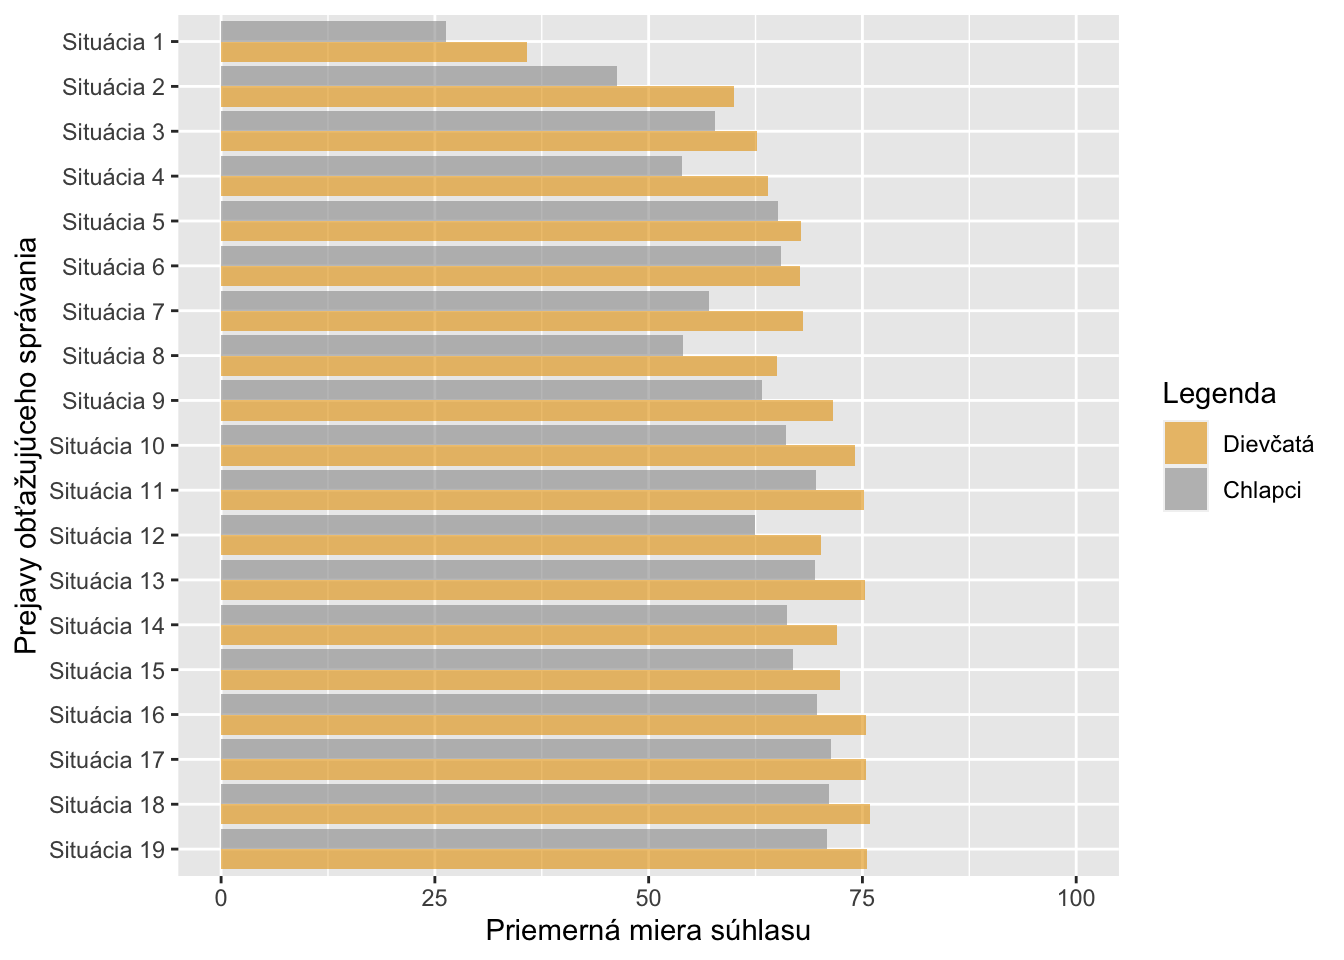
\includegraphics[width=0.8\linewidth,]{_index_files/figure-latex/attPlot-1} 

}

\caption{Miera vnímania sexuálneho obťažovania}\label{fig:attPlot}
\end{figure}

Medzi participantami študujúcimi iné odbory však boli detekované rozdiely, F(5, 1460) = 5.25, p \textless{} .001, BF10 = 61.89. V tabuľke \ref{tab:sensField} je možné vidieť priemery (vyššia hodnota značí vyššiu mieru senzitivity) a smerodajné odchýlky senzitivity na sexuálne obťažovanie naprieč všetkými odbormi. Ako je vidieť v tabuľke regresných koeficinetov \ref{tab:sensFieldReg}, kde odbor ``filozofický, humanitný, pedagogický, teologický'' predstavuje referenčnú skupinu, študenti prírodovedných, technických a zdravotníckych odborov vykazujú v porovnaní so spoločensko-humanitnými odbormi signifikantne nižšiu senzitivitu na sexuálne obťažovanie\footnote{Regresné koeficinety predstavujú rozdiel v priemeroch v porovnaní s referenčnou skupinou (intercept modelu)} filozofických, humanitných, pedagogických, a teologických odborov.{]} Výrazne nižší priemer v porovnaní s referenčnou skupinou bol aj v mediálnych a umeleckých odboroch, no v danom prípade je možné predpokladať nižšiu štatistickú silu na detekciu signifikantného rozdielu z dôvodu malej početnosti participantov tohto odboru vo vzorke.

\begin{table}[H]

\caption{\label{tab:sensField}Senzitivita na sexuálne obťažovanie - deskriptívne charakteristiky}
\centering
\fontsize{10}{12}\selectfont
\begin{tabular}[t]{lrr}
\toprule
Odbor štúdia & M & SD\\
\midrule
\cellcolor{gray!6}{filozofický, humanitný, pedagogický, teologický} & \cellcolor{gray!6}{56.803} & \cellcolor{gray!6}{34.414}\\
mediálny, umelecký & 48.147 & 34.357\\
\cellcolor{gray!6}{prírodovedecký} & \cellcolor{gray!6}{45.857} & \cellcolor{gray!6}{34.586}\\
spoločenský, ekonomický, právny & 59.549 & 31.406\\
\cellcolor{gray!6}{technický} & \cellcolor{gray!6}{51.165} & \cellcolor{gray!6}{33.818}\\
\addlinespace
zdravotnícky & 47.538 & 35.824\\
\bottomrule
\end{tabular}
\end{table}

\begin{table}[H]

\caption{\label{tab:sensFieldReg}Senzitivita na sexuálne obťažovanie - regresný model}
\centering
\resizebox{\linewidth}{!}{
\fontsize{10}{12}\selectfont
\begin{tabular}[t]{lrrrr}
\toprule
  & Beta & SE & t-štatistika & p-hodnota\\
\midrule
\cellcolor{gray!6}{Intercept (filozofický, humanitný, pedagogický, teologický)} & \cellcolor{gray!6}{56.80} & \cellcolor{gray!6}{1.79} & \cellcolor{gray!6}{31.82} & \cellcolor{gray!6}{0.00}\\
mediálny, umelecký & -8.66 & 4.56 & -1.90 & 0.06\\
\cellcolor{gray!6}{prírodovedecký} & \cellcolor{gray!6}{-10.95} & \cellcolor{gray!6}{3.87} & \cellcolor{gray!6}{-2.83} & \cellcolor{gray!6}{0.00}\\
spoločenský, ekonomický, právny & 2.75 & 2.60 & 1.06 & 0.29\\
\cellcolor{gray!6}{technický} & \cellcolor{gray!6}{-5.64} & \cellcolor{gray!6}{2.32} & \cellcolor{gray!6}{-2.43} & \cellcolor{gray!6}{0.02}\\
\addlinespace
zdravotnícky & -9.27 & 3.64 & -2.54 & 0.01\\
\bottomrule
\end{tabular}}
\end{table}

Následne sme testovali, či existuje súvis medzi tým, čo participanti považujú za SO a tým, či majú tendenciou hľadať pomoc, ak sa s niektorou z foriem sexuálneho obťažovania osobne stretli? Táto substantívna otázka bola testovaná regresným modelom kontrolujúcim závažnosť sexuálneho obťažovania. Regresný model\footnote{Prediktormi v modeli boli (1) či sa obeť sexuálneho obťažovania niekomu zdôverila a (2) závažnosť zažitého sexuálneho obťažovania} dokázal robustným spôsobom predikovať senzitivitu voči sexuálnemu obťažovaniu. Aj po zohľadnení závažnosti zažitého sexuálneho obťažovania teda existuje asociácia medzi senzitivitu voči obťažovaniu a tendenciou zdôveriť sa, F(1, 1) = 579.14, p \textless{} .001, BF10 = 512.66.

\begin{table}[H]

\caption{\label{tab:unnamed-chunk-6}Senzitivita na sexuálne obťažovanie a zdôverenie sa}
\centering
\fontsize{10}{12}\selectfont
\begin{tabular}[t]{lrr}
\toprule
  & M & SD\\
\midrule
\cellcolor{gray!6}{Participant sa nezdôveril} & \cellcolor{gray!6}{49.9} & \cellcolor{gray!6}{34.4}\\
Participant sa zdôveril & 59.8 & 31.6\\
\cellcolor{gray!6}{Participant nebol obeťou obťažovania} & \cellcolor{gray!6}{56.2} & \cellcolor{gray!6}{33.8}\\
\bottomrule
\end{tabular}
\end{table}

Na druhej strane sa nepreukázal empiricky robustný vzťah medzi senzitivitou voči sexuálnemu obťažovaniu a (1) regiónom odkiaľ obete pochádzajú, F(2, 1463) = 1.5, p = 0.22, BF10 = 7, alebo (2) vierovyznaním participanta, F(1, 1464) = 0.77, p = 0.38, BF01 = 9.79.

\hypertarget{stereotypy-o-sexuuxe1lnom-obux165aux17eovanuxed}{%
\subsection{Stereotypy o sexuálnom obťažovaní}\label{stereotypy-o-sexuuxe1lnom-obux165aux17eovanuxed}}

V závere výskumu bolo participantom administrovaných 11 výrokov reprezentujúcich miskoncepcie o sexuálnom obťažovaní. Ich zoznam je uvedený v Tabuľke \ref{tab:miscList}).

\begin{table}[H]

\caption{\label{tab:miscList}Zoznam miskonceptov o sexuálnom obťažovaní}
\centering
\resizebox{\linewidth}{!}{
\fontsize{10}{12}\selectfont
\begin{tabular}[t]{ll}
\toprule
 & Formulácia miskonceptu\\
\midrule
\cellcolor{gray!6}{Miskoncept 1} & \cellcolor{gray!6}{Ženy si často vymýšľajú obvinenia zo sexuálneho obťažovania.}\\
Miskoncept 2 & Vyučujúci / vyučujúce by nemali mať romantické vzťahy so svojimi študentmi / študentkami.\\
\cellcolor{gray!6}{Miskoncept 3} & \cellcolor{gray!6}{Vyučujúci / vyučujúce by nemali mať sexuálne vzťahy so svojimi študentmi / študentkami.}\\
Miskoncept 4 & Sexuálne obťažovanie je zneužitie, ktoré ovplyvňuje kvalitu života osoby, na ktorej je páchané.\\
\cellcolor{gray!6}{Miskoncept 5} & \cellcolor{gray!6}{Keď sa bude sexuálne obťažovanie ignorovať, prestane.}\\
\addlinespace
Miskoncept 6 & Ľudia, ktorí zažili sexuálne obťažovanie, ale rozhodnú sa ho nahlásiť až po rokoch, nemajú nárok na spravodlivoť (napr. potrestanie vinníka).\\
\cellcolor{gray!6}{Miskoncept 7} & \cellcolor{gray!6}{Ženy, ktoré sa obliekajú sexuálne atraktívnym spôsobom si koledujú o sexuálnu pozornosť (napr. komentáre).}\\
Miskoncept 8 & Muži, ktorí sa obliekajú sexuálne atraktívnym spôsobom si koledujú o sexuálnu pozornosť (napr. komentáre).\\
\cellcolor{gray!6}{Miskoncept 9} & \cellcolor{gray!6}{Zodpovednosť za sexuálne obťažovanie prináleží v plnej miere osobe, ktorá sa obťažovania dopúšťa, bez ohľadu na vzhľad alebo konanie osoby, ktorá je obťažovaná.}\\
Miskoncept 10 & So sexuálnym obťažovaním sa nedá nič robiť.\\
\addlinespace
\cellcolor{gray!6}{Miskoncept 11} & \cellcolor{gray!6}{Vedenie školy by malo prijať opatrenia na predchádzanie sexuálneho obťažovania.}\\
\bottomrule
\end{tabular}}
\end{table}

Na grafe \ref{fig:miscPlot} je zobrazená priemerná miera súhlasu s miskonceptmi o sexuálnom obťažovaní separátne pre dievčatá a chlapcov. Priemerné miery súhlasu s danými tvrdeniami pomerne konzistentne indikujú mierne vyššiu mieru miskoncepcií o sexuálnom obťažovaní v aktuálnej vzorke chlapcov. V celkovej miere súhlasu s miskonceptami\footnote{Celková miera súhlasu s miskoncepciami o sexuálnom obťažovaní bola vypočítaná ako nevážený súčet skóre jednotlivých položiek po preškálovaní inverzných položiek č. 2, 3, 4, 9, 11.} však medzi pohlaviami nebol zistený štatisticky signifikantný rozdiel, F(1, 1442) = 3.11, p = 0.08, BF01 = 3.6. Jediný štatisticky signifikantný rozdiel v miere akceptácie miskonceptov bol zistený v závislosti od regiónu, z ktorého participantami pochádzali, no miera dôkazov v prospech tohto efektu prakticky absentovala, F(2, 1463) = 3.77, p = 0.02, BF01 = 74.91.

\begin{figure}

{\centering 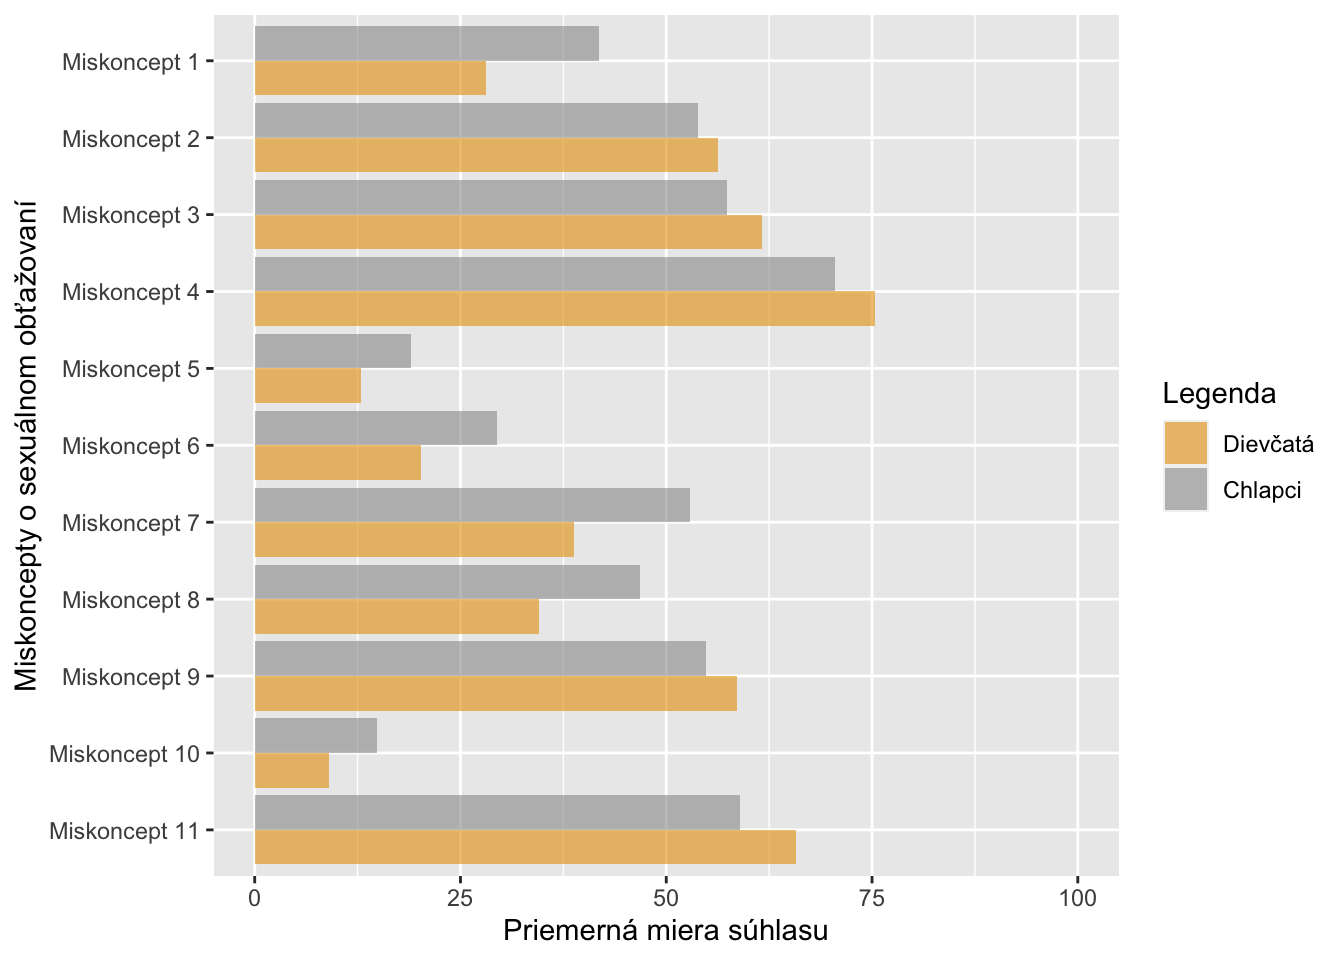
\includegraphics[width=0.8\linewidth,]{_index_files/figure-latex/miscPlot-1} 

}

\caption{Miera súhlasu s miskonceptmi o sexuálnom obťažovaní}\label{fig:miscPlot}
\end{figure}

Exaktné distribúcie odpovedí na položky merajúce miskoncepty o sexuálnom obťažovaní jednotlivo pre dievčatá a chlapcov sú zobrazené v Tabuľkách \ref{tab:miscF}, resp. \ref{tab:miscM}.

\begin{table}[H]

\caption{\label{tab:miscF}Distribúcia odpovedí u dievčat}
\centering
\resizebox{\linewidth}{!}{
\fontsize{10}{12}\selectfont
\begin{tabular}[t]{lrrrrr}
\toprule
  & Úplne nesúhlasím & Skôr nesúhlasím & Neviem & Skôr súhlasím & Úplne súhlasím\\
\midrule
\cellcolor{gray!6}{Miskoncept 1} & \cellcolor{gray!6}{13.07} & \cellcolor{gray!6}{49.58} & \cellcolor{gray!6}{23.37} & \cellcolor{gray!6}{11.75} & \cellcolor{gray!6}{2.22}\\
Miskoncept 2 & 3.21 & 13.39 & 15.77 & 34.03 & 33.60\\
\cellcolor{gray!6}{Miskoncept 3} & \cellcolor{gray!6}{3.26} & \cellcolor{gray!6}{9.30} & \cellcolor{gray!6}{13.28} & \cellcolor{gray!6}{24.07} & \cellcolor{gray!6}{50.09}\\
Miskoncept 4 & 0.34 & 0.71 & 2.40 & 15.02 & 81.54\\
\cellcolor{gray!6}{Miskoncept 5} & \cellcolor{gray!6}{58.27} & \cellcolor{gray!6}{27.27} & \cellcolor{gray!6}{7.68} & \cellcolor{gray!6}{5.33} & \cellcolor{gray!6}{1.45}\\
\addlinespace
Miskoncept 6 & 43.78 & 26.37 & 18.29 & 8.01 & 3.55\\
\cellcolor{gray!6}{Miskoncept 7} & \cellcolor{gray!6}{20.90} & \cellcolor{gray!6}{20.78} & \cellcolor{gray!6}{12.51} & \cellcolor{gray!6}{35.25} & \cellcolor{gray!6}{10.56}\\
Miskoncept 8 & 21.37 & 27.28 & 15.35 & 29.43 & 6.57\\
\cellcolor{gray!6}{Miskoncept 9} & \cellcolor{gray!6}{2.27} & \cellcolor{gray!6}{12.29} & \cellcolor{gray!6}{16.84} & \cellcolor{gray!6}{27.35} & \cellcolor{gray!6}{41.25}\\
Miskoncept 10 & 66.07 & 26.24 & 5.04 & 1.71 & 0.94\\
\addlinespace
\cellcolor{gray!6}{Miskoncept 11} & \cellcolor{gray!6}{2.42} & \cellcolor{gray!6}{2.24} & \cellcolor{gray!6}{9.70} & \cellcolor{gray!6}{35.17} & \cellcolor{gray!6}{50.47}\\
\bottomrule
\end{tabular}}
\end{table}

\begin{table}[H]

\caption{\label{tab:miscM}Distribúcia odpovedí u chlapcov}
\centering
\resizebox{\linewidth}{!}{
\fontsize{10}{12}\selectfont
\begin{tabular}[t]{lrrrrr}
\toprule
  & Úplne nesúhlasím & Skôr nesúhlasím & Neviem & Skôr súhlasím & Úplne súhlasím\\
\midrule
\cellcolor{gray!6}{Miskoncept 1} & \cellcolor{gray!6}{3.02} & \cellcolor{gray!6}{25.81} & \cellcolor{gray!6}{38.08} & \cellcolor{gray!6}{25.40} & \cellcolor{gray!6}{7.69}\\
Miskoncept 2 & 5.17 & 13.96 & 14.20 & 40.03 & 26.64\\
\cellcolor{gray!6}{Miskoncept 3} & \cellcolor{gray!6}{2.93} & \cellcolor{gray!6}{13.91} & \cellcolor{gray!6}{12.43} & \cellcolor{gray!6}{35.08} & \cellcolor{gray!6}{35.65}\\
Miskoncept 4 & 0.13 & 1.89 & 7.22 & 26.84 & 63.92\\
\cellcolor{gray!6}{Miskoncept 5} & \cellcolor{gray!6}{39.80} & \cellcolor{gray!6}{36.98} & \cellcolor{gray!6}{14.50} & \cellcolor{gray!6}{6.11} & \cellcolor{gray!6}{2.61}\\
\addlinespace
Miskoncept 6 & 24.11 & 32.98 & 22.65 & 11.94 & 8.33\\
\cellcolor{gray!6}{Miskoncept 7} & \cellcolor{gray!6}{7.12} & \cellcolor{gray!6}{13.31} & \cellcolor{gray!6}{13.99} & \cellcolor{gray!6}{39.47} & \cellcolor{gray!6}{26.11}\\
Miskoncept 8 & 9.58 & 17.76 & 17.15 & 39.82 & 15.69\\
\cellcolor{gray!6}{Miskoncept 9} & \cellcolor{gray!6}{3.70} & \cellcolor{gray!6}{13.07} & \cellcolor{gray!6}{17.11} & \cellcolor{gray!6}{37.45} & \cellcolor{gray!6}{28.67}\\
Miskoncept 10 & 48.63 & 35.73 & 9.51 & 4.76 & 1.37\\
\addlinespace
\cellcolor{gray!6}{Miskoncept 11} & \cellcolor{gray!6}{1.24} & \cellcolor{gray!6}{6.30} & \cellcolor{gray!6}{21.17} & \cellcolor{gray!6}{39.23} & \cellcolor{gray!6}{32.05}\\
\bottomrule
\end{tabular}}
\end{table}

Rovnako nebola zistená systematická asociácia medzi celkovou mierou akceptácie miskonceptov a vekom participantov, F(1, 1444) = 0.21, p = 0.64, BF01 = 4.97, ich odborom štúdia, F(5, 1460) = 1.86, p = 0.1, BF01 = 241.18, či ich vierovyznaním, F(1, 1464) = 3.84, p = 0.05, BF01 = 5.57. Zároveň bolo testované, či osoby, ktoré majú viac skúseností so sexuálnym obťažovaním zvyknú aj viac situácií vyhodnocovať ako obťažujúce správanie. U obetí obťažovania však nebola detekovaná výrazne nižšia miera akceptácie miskonceptov, F(1, 1464) = 2.04, p = 0.15, BF01 = 2.97. Rozdiel v miere akceptácie miskonceptov nebol ani medzi obeťami, ktoré sa zdôverili a tými, čo sa nezdôverili, F(1, 1) = 847.97, p \textless{} .001, BF01 = 131.21.

\newpage

\hypertarget{referencie}{%
\section{Referencie}\label{referencie}}

Gunel, E., \& Dickey, J. (1974). Bayes factors for independence in contingency tables. Biometrika, 61(3), 545--557. \url{doi:10.1093/biomet/61.3.545}

Jamil, T., Ly, A., Morey, R. D., Love, J., Marsman, M., \& Wagenmakers, E.-J. (2016). Default ``Gunel and Dickey'' Bayes factors for contingency tables. Behavior Research Methods, 49(2), 638--652. \url{doi:10.3758/s13428-016-0739-8}

Jeffreys, H. (1961). Theory of probability. Oxford University Press: Oxford UK.

Meade, A. W., \& Craig, S. B. (2012). Identifying careless responses in survey data. Psychological Methods, 17(3), 437--455. \url{doi:10.1037/a0028085}

Rothman, K. J., \& Greenland, S. (1998). Modern Epidemiology. Lippincott-Raven Publishers

Wagenmakers, E.-J. (2007). A practical solution to the pervasive problems ofp values. Psychonomic Bulletin \& Review, 14(5), 779--804. \url{doi:10.3758/bf03194105}

\end{document}
